\chapter{観測データ解析 \label{chapObs}}

% Chap.4 観測データを用いたオールト解析 (仮)
% 4.1 使用する観測データ
%  4.1.1 観測データのカタログ ← Sanders & Das (2018) の説明
%  4.1.2 解析に使用するサンプル選定
% 4.2 観測データの解析結果 (仮)


% Chap. 4 観測データの解析結果
% ここもあとで議論しながら整理しましょう。
% ここの解析ではSgrA*のVLBI観測値である太陽の回転速度をfixしていると思います。
% この場合、MCMC解析にもちいる尤度関数はChap.3にあったものと変わっていませんか?
% 違うなら、ここにもちゃんと利用した尤度関数 (解析手法) を書きましょう。

第\ref{chapMock}章では模擬データの解析からasymmetric driftなどの効果の影響を調べた。以上の結果を踏まえて、観測データの解析を行う。\ref{観測データ}では、本論文の解析で用いた観測データについて説明する。\ref{使用するサンプル}では観測データの中から実際に解析で使用するサンプルについて説明する。\ref{観測データの解析結果}では、そのように選んできたサンプルを解析した結果を記述する。

\section{観測データ \label{観測データ}}
本研究では\cite{SD18}のカタログを用いて観測データの解析を行っている。このカタログはAPOGEE, Gaia-DSO, GALAH, LAMOST, RAVE, SEGUEの分光サーベイから利用できる分光パラメータとGaia Data Release 2 (DR2)で観測されたデータから約300万天体の年齢推定値を含むカタログとなっている。表\ref{spec_dataset}は彼らがカタログ生成の際に用いた分光データセットの表である。図\ref{fig2}は\cite{SD18}で年齢推定をした星の銀河座標系での分布である。

\cite{SD18}は等時曲線フィットにより分光データから年齢推定を行っており、年齢の不定性はAPOGEEで$\sim 16\,\%$(最も正確な分光年齢推定)、GALAHで$\sim 21\,\%$、LAMOSTで$\sim 25\,\%$、RAVEとGESで$\sim 40\,\%$となっている。等時曲線とは、恒星進化の理論から与えられる年齢一定の星をヘルツシュプルング・ラッセル図 (HR図) 上でプロットしたときに結んだ線のことである。この等時曲線を、観測した星のHR図上での分布に対してフィッティングをすることで年齢推定をする方法が等時曲線フィットである。
\begin{table}[htb]
\small
\begin{center}
\scalebox{0.87}[0.9]{
\begin{tabular}{|l||c|c|c|c|c|} \hline
    観測 & 天体数 & 波長 & 分解能 & 使用したパラメータ & 測光データ\\ \hline
    APOGEE & 250万 & $H$バンド 15200 - 16900\AA & 22500 & $T_{\mathrm{eff}},\log g, \mathrm{[M/H]}$ & 2MASS\\
    LAMOST & 310万 & 可視光(3650 - 9000 \AA) & 1800 & $T_{\mathrm{eff}},\log g, \mathrm{[Fe/H]}$ & 2MASS \\
    RAVE & 50万 & 8400 - 8800 \AA & 7500 &   & 2MASS\\
    GES & & & 20000, 50000 & $T_{\mathrm{eff}},\log g, \mathrm{[Fe/H]}$ & VISTA, 2MASS\\
    GALAH & 26万 &  & 28000 & $T_{\mathrm{eff}},\log g, \mathrm{[Fe/H]}$ & 2MASS\\
    SEGUE & 19万 & 可視光 & 2000 & $T_{\mathrm{eff}},\log g, \mathrm{[Fe/H]}$ & 2MASS\\ \hline
\end{tabular}
}
\caption{\cite{SD18}のカタログで用いられた分光観測の種類、それぞれのデータの天体数、波長、分解能、年齢推定に使用したパラメータと測光データ。}
\end{center} \label{spec_dataset}
\end{table}

\begin{figure*}[htbp]
\begin{center}
	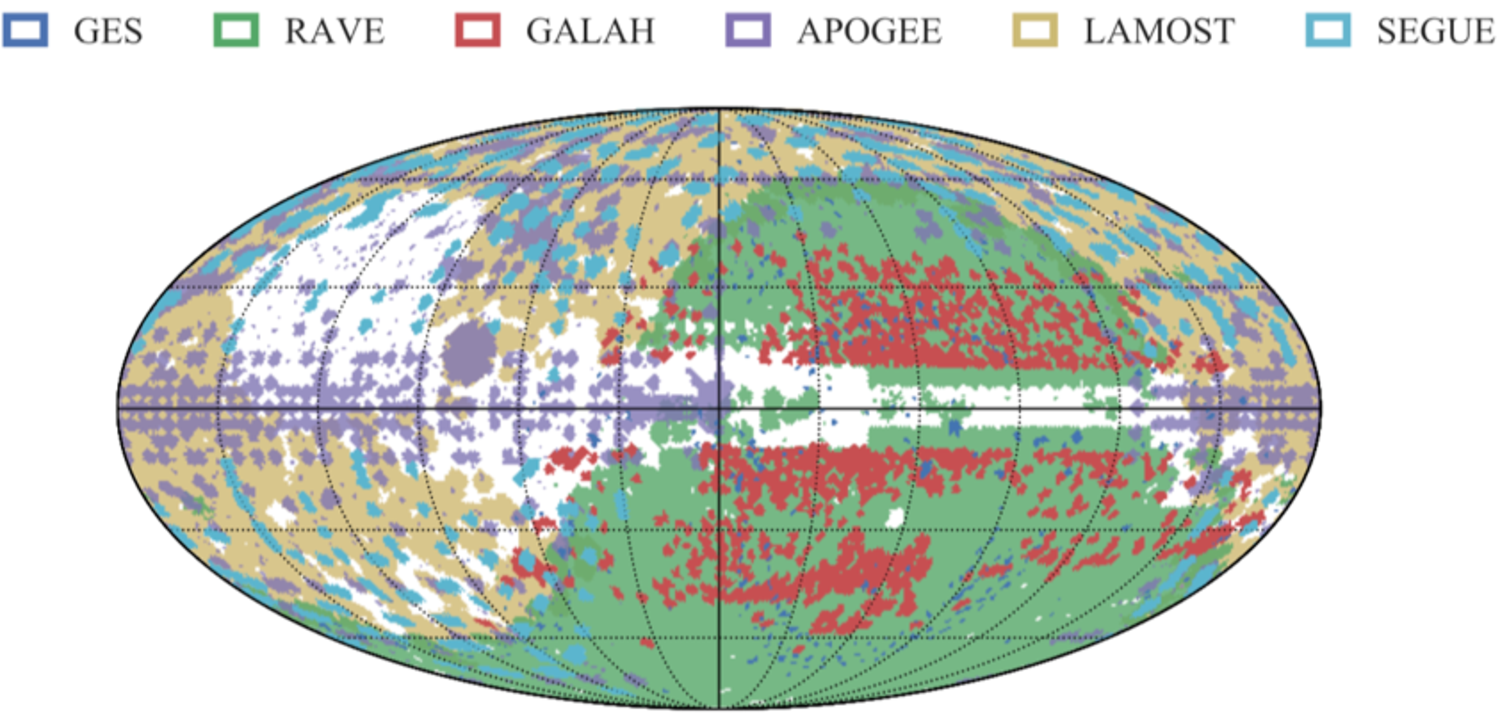
\includegraphics[width=9cm]{fig/SD18_fig1.pdf}
	\caption{\cite{SD18}で年齢推定がなされた星の分布。銀河を見たときのサーベイごとに色付けしている。}
	\label{fig2}
\end{center}
\end{figure*}

図\ref{mode_plx}、\ref{mode_plx-age}はそれぞれ本研究で使用しているサンプルの年周視差$\varpi$ごとのモードと星の年齢$\tau$ごとのモードである。モードが大きすぎるとモードミキシングを起こしてしまうため、モードが大きくないかどうかを確かめる必要がある。例えば、年周視差$\varpi$がモード1を持っていると太陽運動$U_{\odot}、V_{\odot}、W_{\odot}$に、モード2を持っているとオールト定数$A、B、C、K$に影響してしまう。図\ref{mode_plx}の年周視差ごとのモードでは、$0<\varpi<2\,\si{mas}$では1のモードが-50\%、2のモードが約40\%と大きくなっていることがわかる。$2<\varpi<4\,\si{mas}$、$4<\varpi<6\,\si{mas}$でも1、2のモードの絶対値が約20\%以上と比較的大きい。

\begin{figure*}[htbp]
\begin{center}
	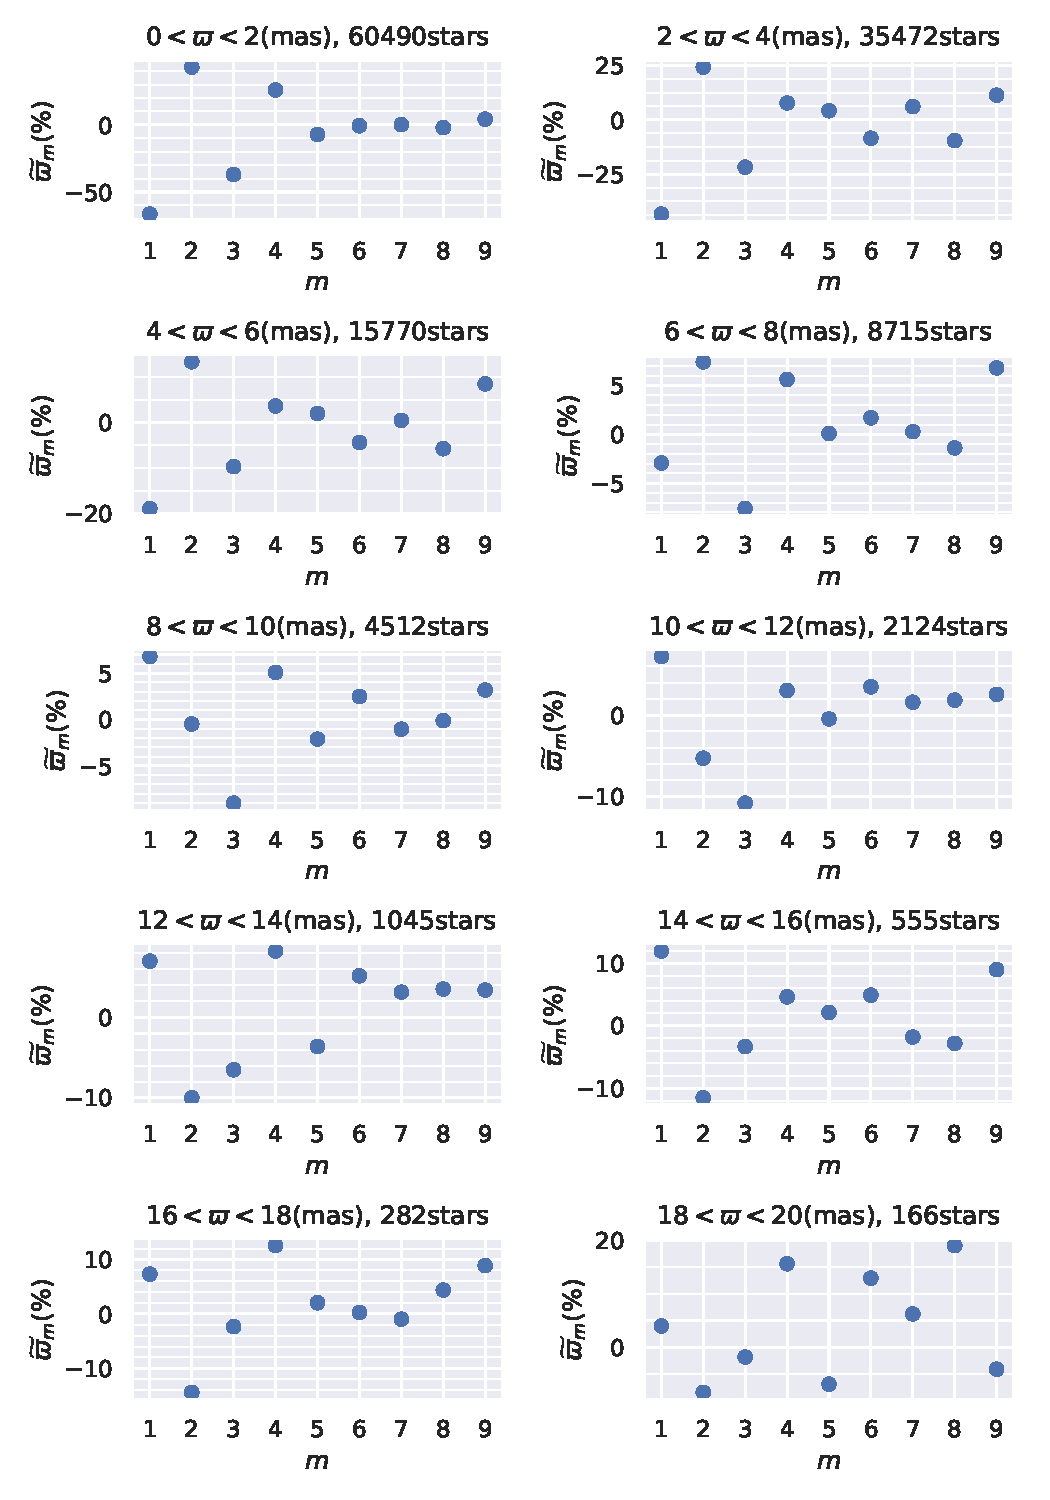
\includegraphics[width=12cm]{fig/mode_plx.pdf}
	\caption{今回使用しているサンプルの年周視差2 masごとのモード。各年周視差ごとのサンプルをフーリエ変換している。mはモードの係数である。}
	\label{mode_plx}
\end{center}
\end{figure*}

\begin{figure*}[htbp]
\begin{center}
	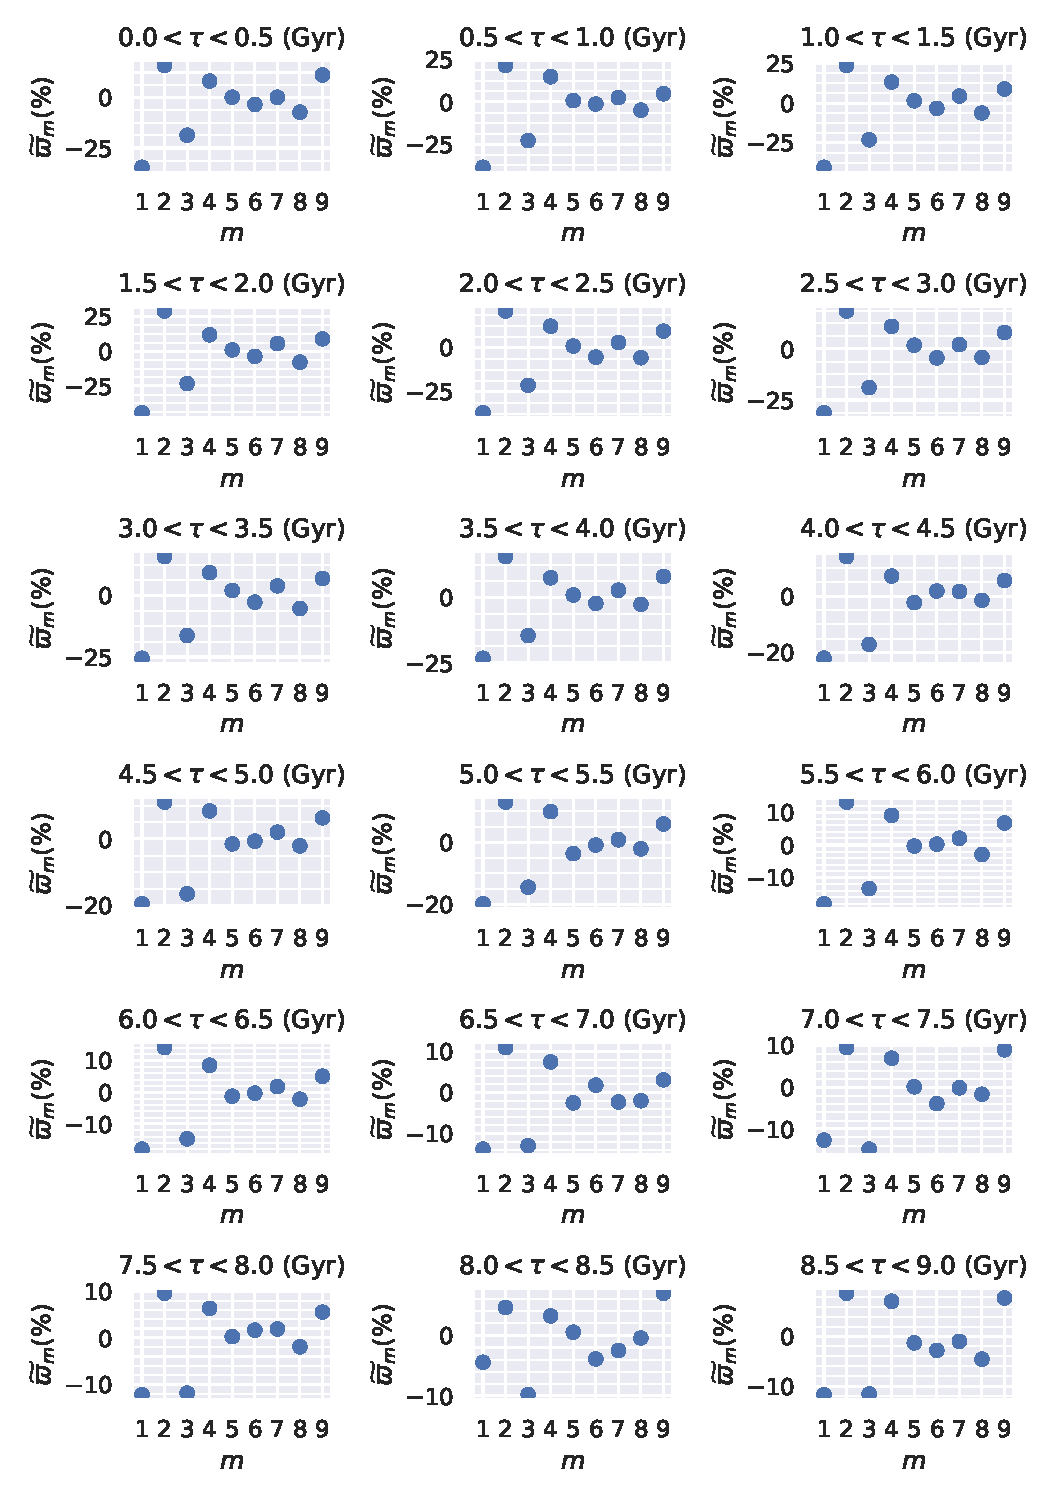
\includegraphics[width=14cm]{fig/mode_plx-age.pdf}
	\caption{太陽から1 kpc以内、年周視差の精度20\%以上、速度の観測誤差$3\,\mathrm{km\,s^{-1}}$以下の星の年齢0 Gyrから9 Gyrまでの0.5 Gyrごとのサンプルの年齢ごとのモード。mはモードの係数である。}
	\label{mode_plx-age}
\end{center}
\end{figure*}

図\ref{hist_seaborn_50Myr}, \ref{hist_seaborn_200Myr}, \ref{hist_seaborn_1Gyr}は星の年齢ごとの$U,V$の2次元速度分布である。$|z|<100\ \mathrm{pc}$のサンプルを使用している。

\begin{figure*}[htbp]
\begin{center}
	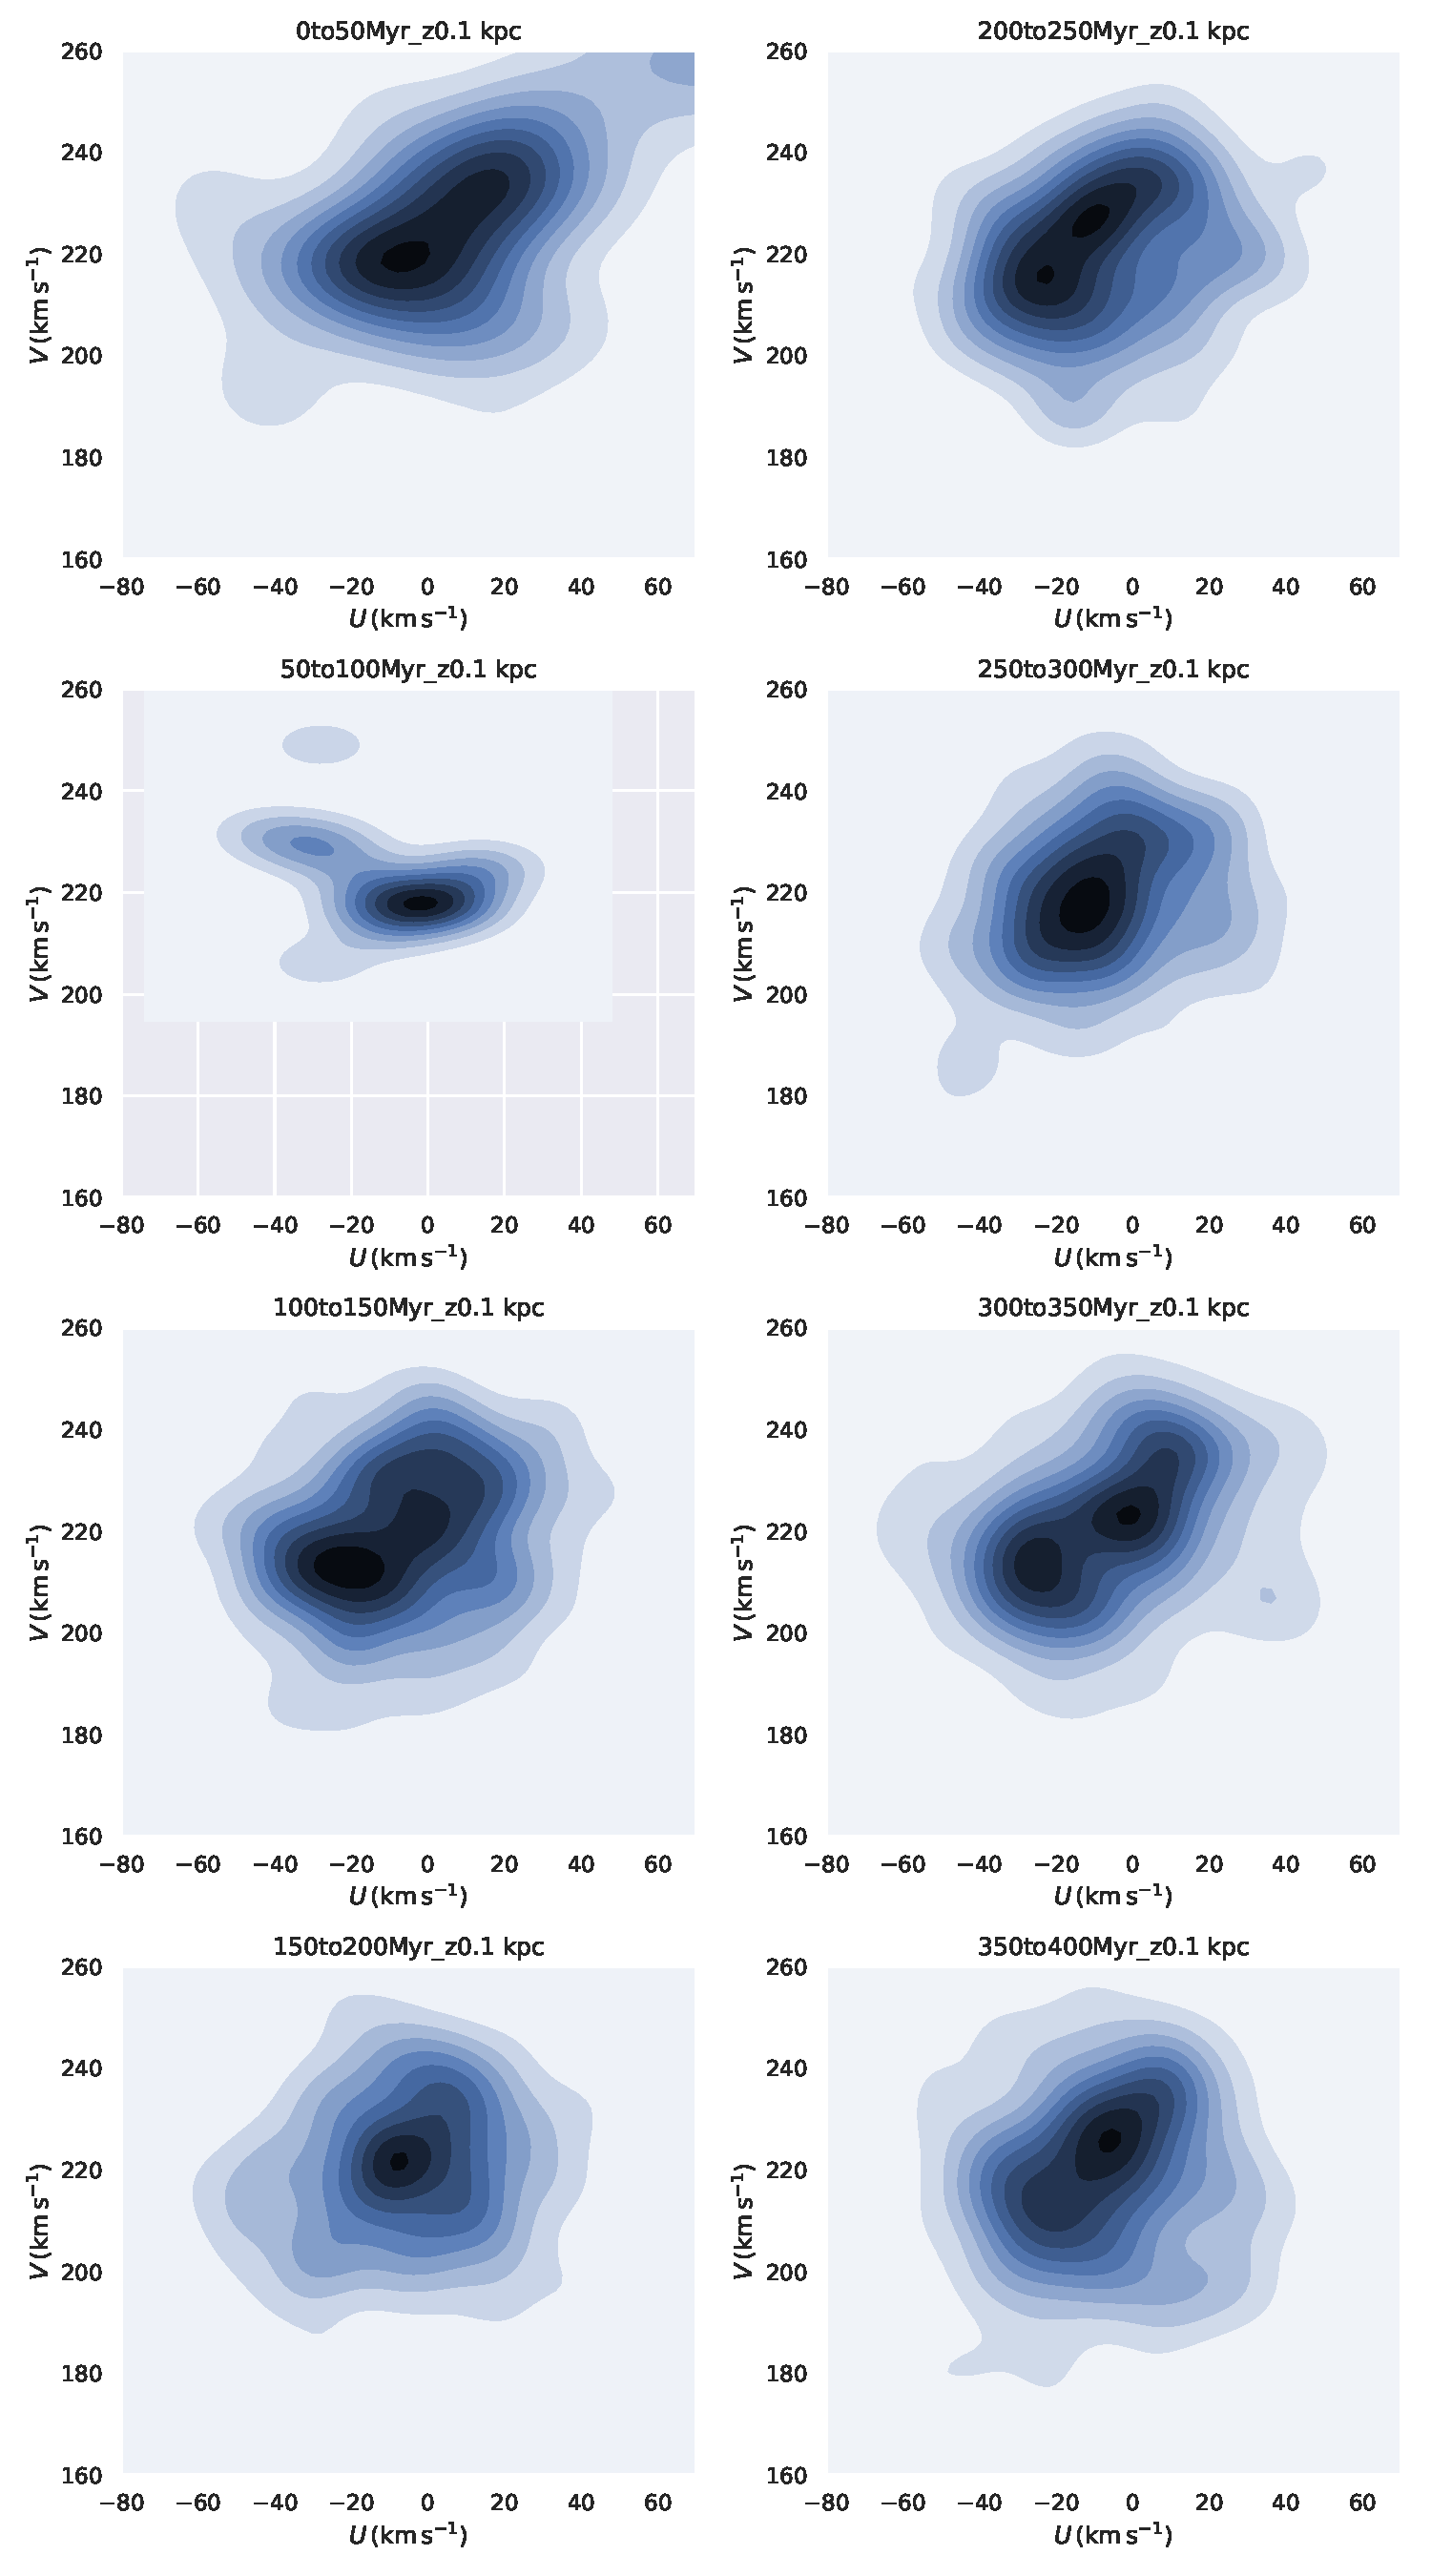
\includegraphics[width=12cm]{fig/UV/hist_seaborn_2_z0.1kpc.pdf}
	\caption{太陽から1 kpc以内、年周視差の精度20\%以上、速度の観測誤差$3\,\mathrm{km\,s^{-1}}$以下の星の年齢50 Myrごとの動径方向速度$U$、方位角方向速度$V$の分布。}
	\label{hist_seaborn_50Myr}
\end{center}
\end{figure*}

\begin{figure*}[htbp]
\begin{center}
	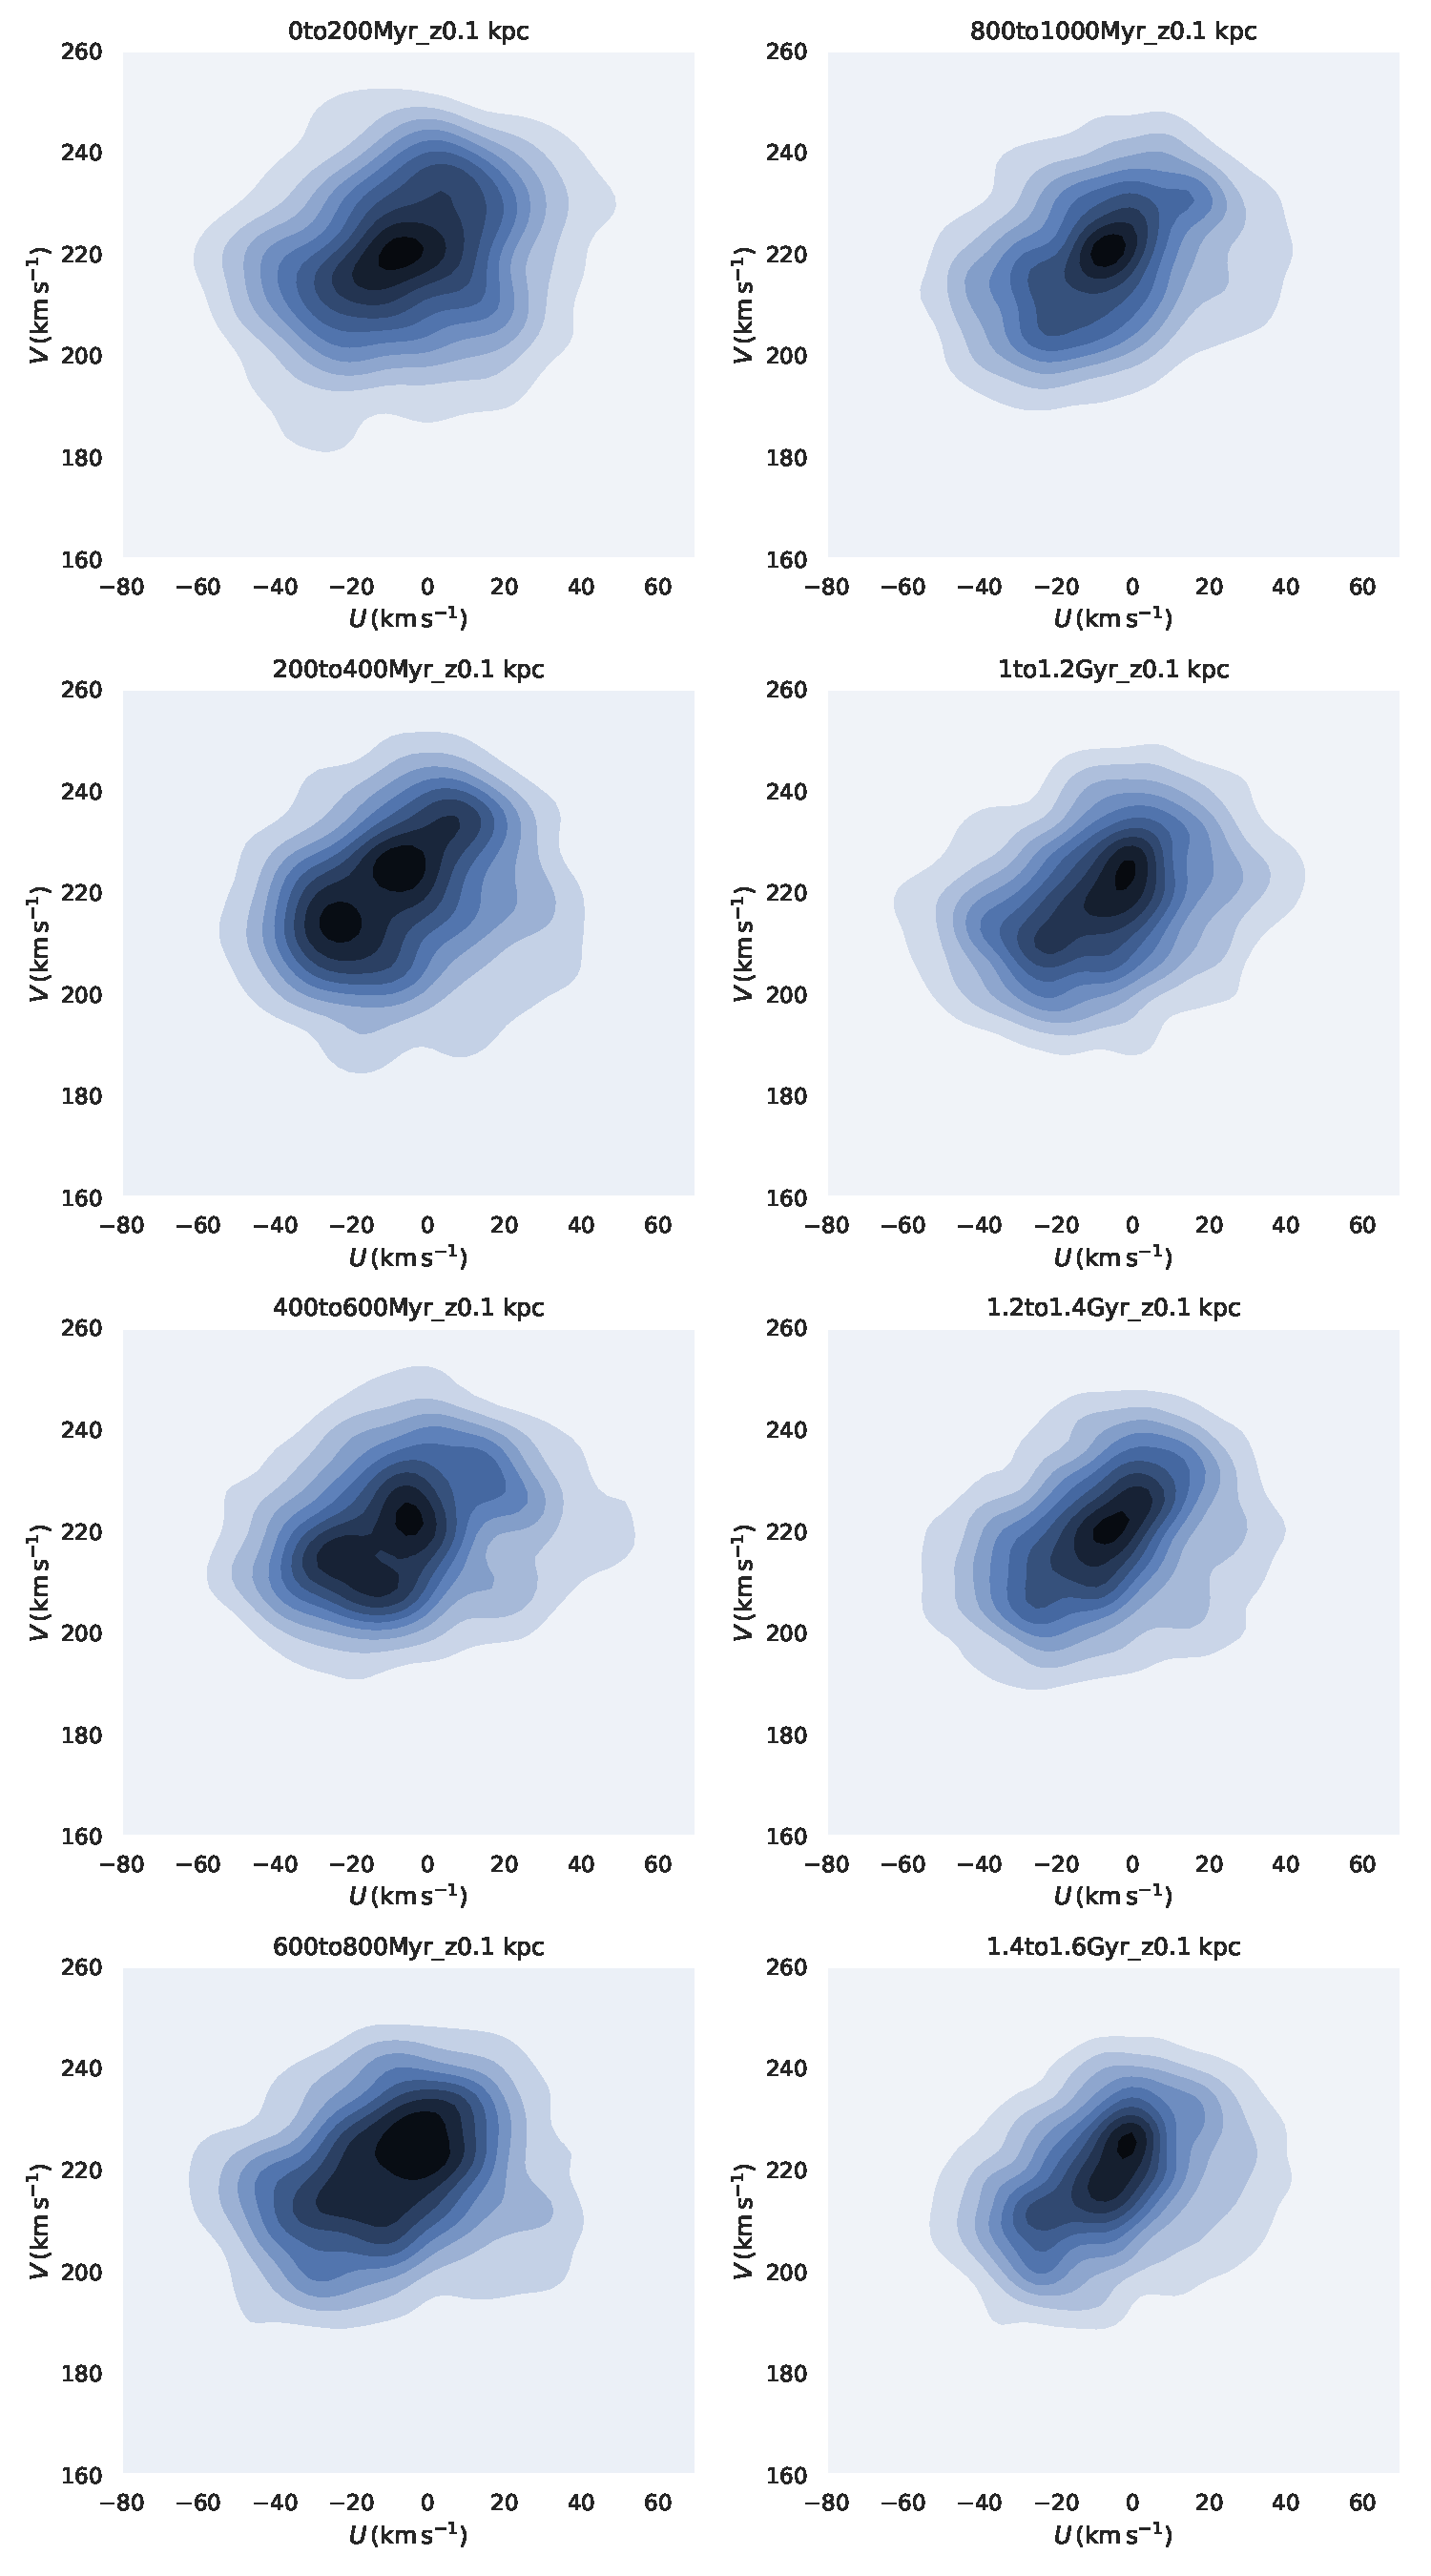
\includegraphics[width=12cm]{fig/UV/hist_seaborn_1_z0.1kpc.pdf}
	\caption{太陽から1 kpc以内、年周視差の精度20\%以上、速度の観測誤差$3\,\mathrm{km\,s^{-1}}$以下の星の年齢200 Myrごとの動径方向速度$U$、方位角方向速度$V$の分布。}
	\label{hist_seaborn_200Myr}
\end{center}
\end{figure*}

\begin{figure*}[htbp]
\begin{center}
	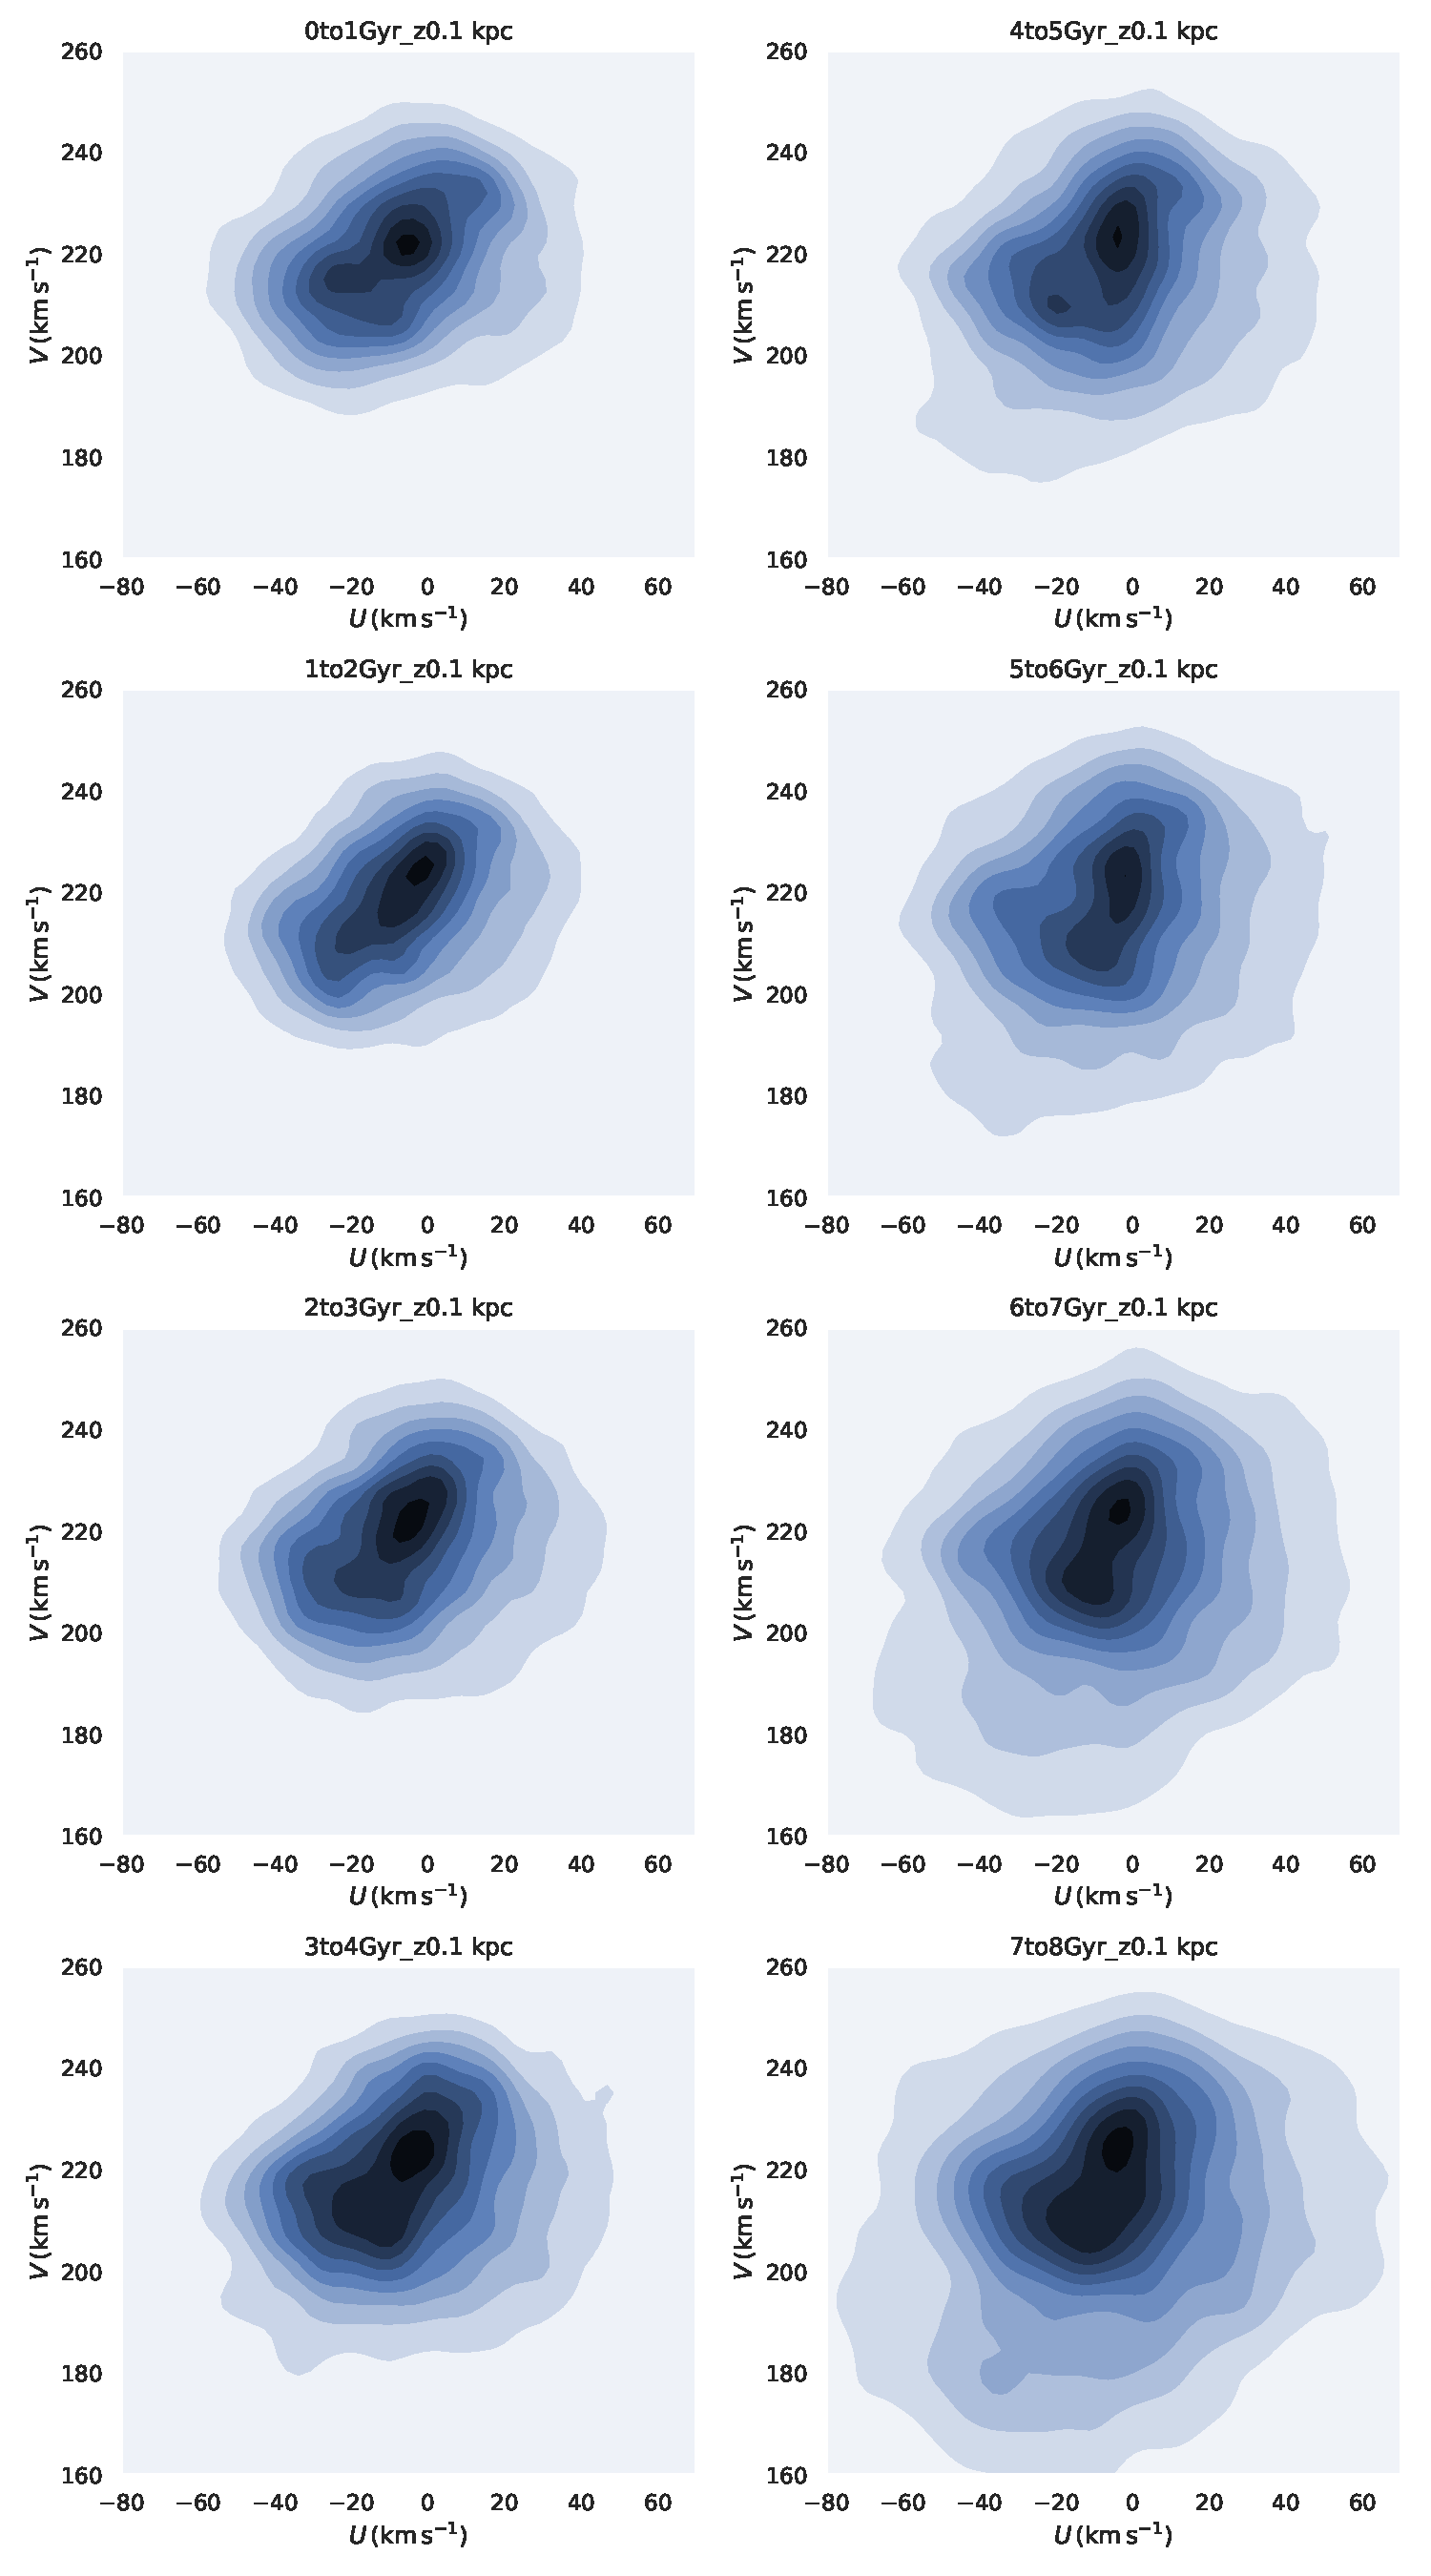
\includegraphics[width=12cm]{fig/UV/hist_seaborn_0_z0.1kpc.pdf}
	\caption{太陽から1 kpc以内、年周視差の精度20\%以上、速度の観測誤差$3\,\mathrm{km\,s^{-1}}$以下の星の年齢1 Gyrごとの動径方向速度$U$、方位角方向速度$V$の分布。}
	\label{hist_seaborn_1Gyr}
\end{center}
\end{figure*}

図\ref{hist_UV_50Myr}, \ref{hist_UV_200Myr}, \ref{hist_UV_1Gyr}は図\ref{hist_seaborn_50Myr}, \ref{hist_seaborn_200Myr}, \ref{hist_seaborn_1Gyr}をプロット方法を変えてプロットした図である。

\begin{figure*}[htbp]
   \centering
\begin{tabular}{cc}
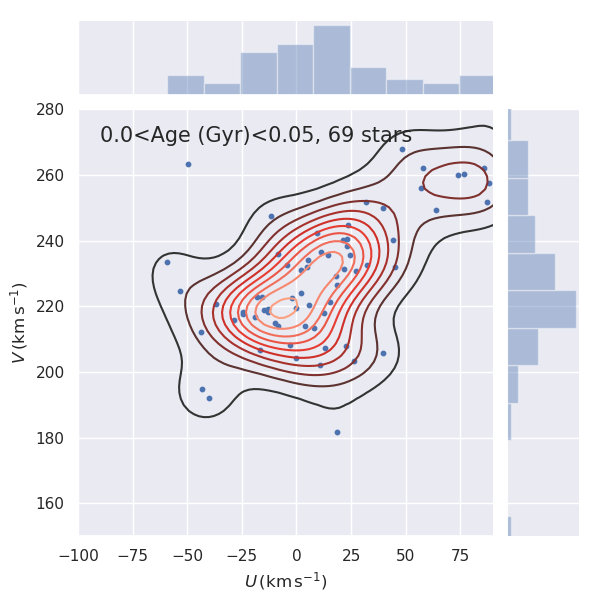
\includegraphics[width=5cm]{fig/UV/0to50Myr_z0.1kpc_hist2d.png}&
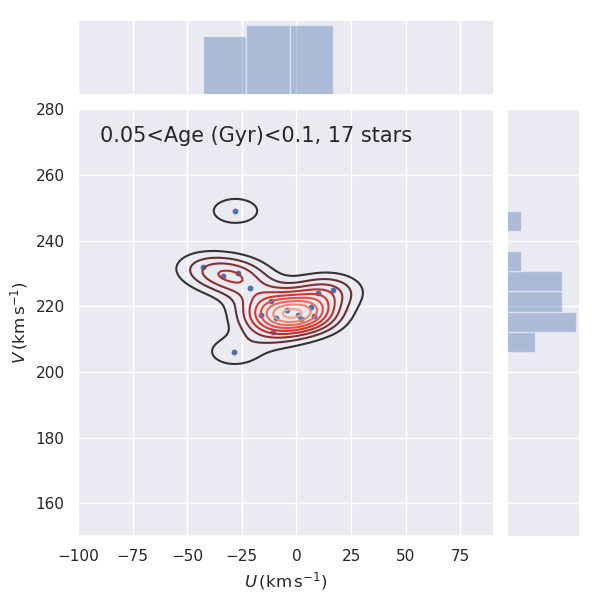
\includegraphics[width=5cm]{fig/UV/50to100Myr_z0.1kpc_hist2d.png}\\
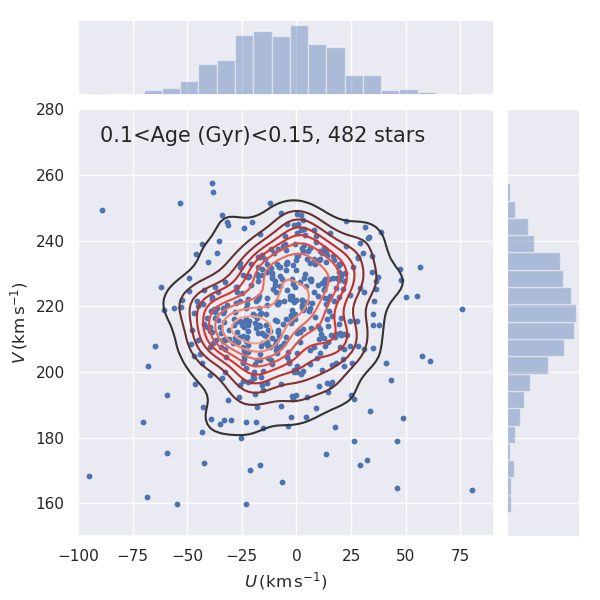
\includegraphics[width=5cm]{fig/UV/100to150Myr_z0.1kpc_hist2d.png}&
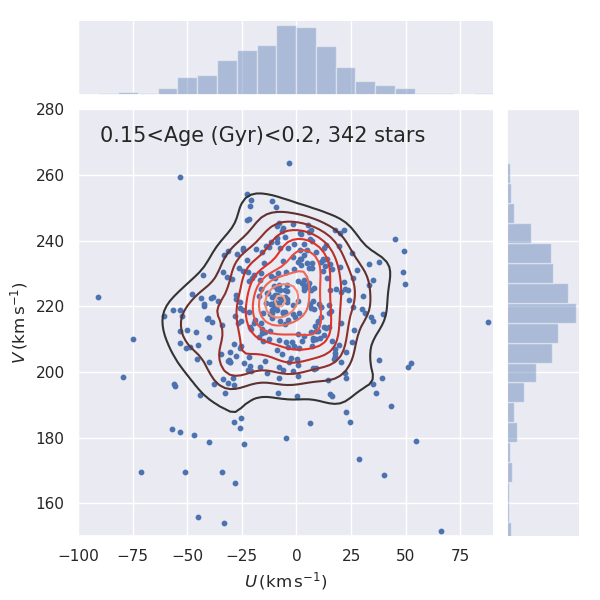
\includegraphics[width=5cm]{fig/UV/150to200Myr_z0.1kpc_hist2d.png}\\
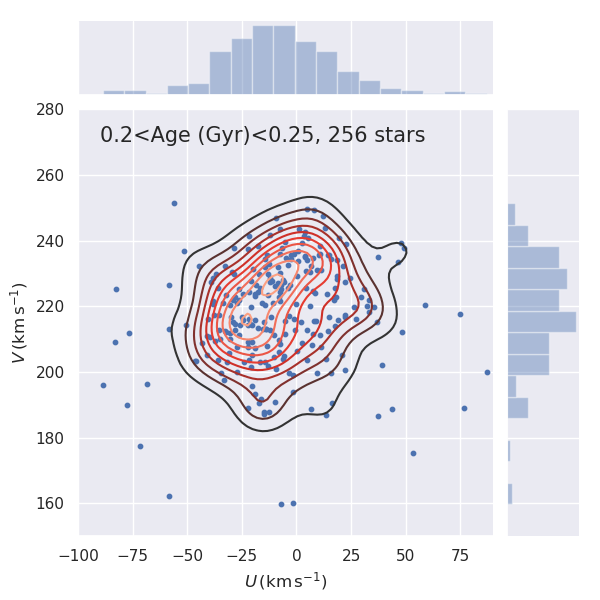
\includegraphics[width=5cm]{fig/UV/200to250Myr_z0.1kpc_hist2d.png}&
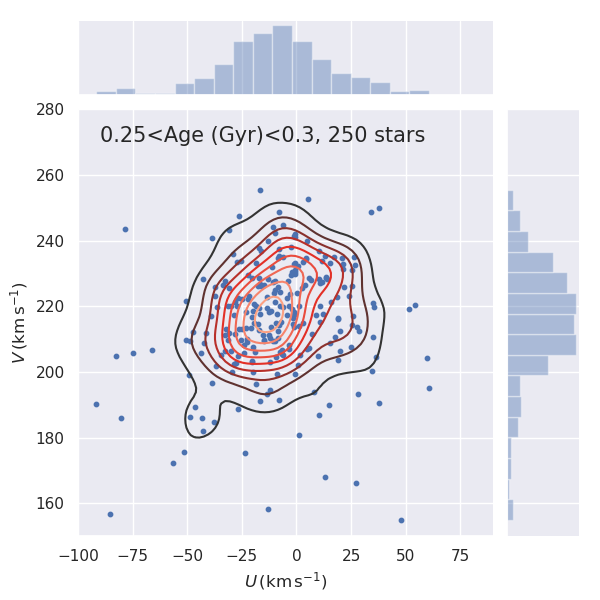
\includegraphics[width=5cm]{fig/UV/250to300Myr_z0.1kpc_hist2d.png}\\
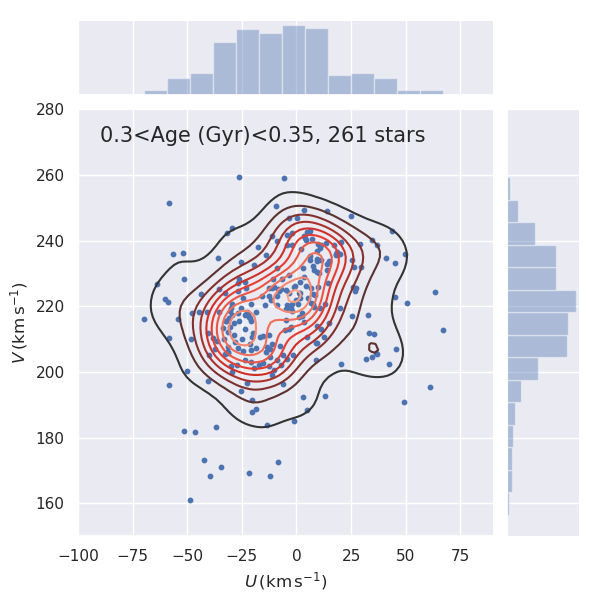
\includegraphics[width=5cm]{fig/UV/300to350Myr_z0.1kpc_hist2d.png}&
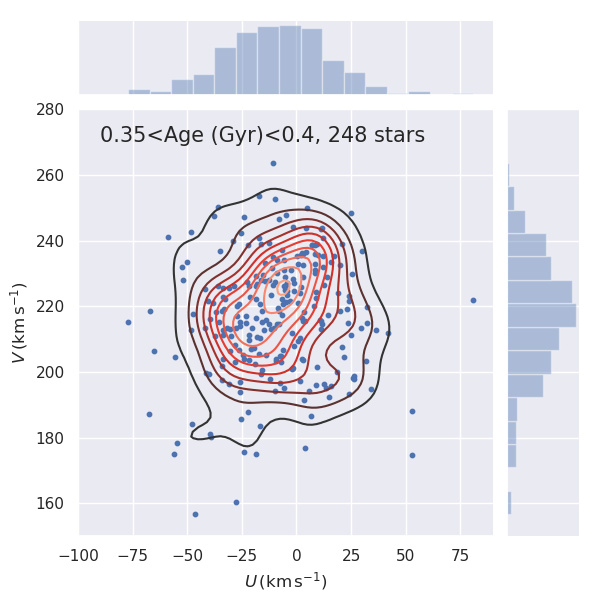
\includegraphics[width=5cm]{fig/UV/350to400Myr_z0.1kpc_hist2d.png}\\
\end{tabular}
    \caption{太陽から1 kpc以内、年周視差の精度20\%以上、速度の観測誤差$3\,\mathrm{km\,s^{-1}}$以下の星の年齢50 Myrごとの動径方向速度$U$、方位角方向速度$V$の分布。}
    \label{hist_UV_50Myr}
\end{figure*}

\begin{figure*}[htbp]
   \centering
\begin{tabular}{cc}
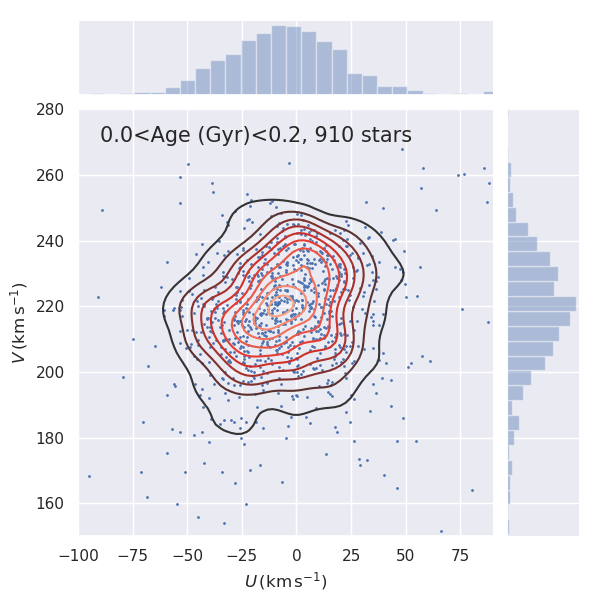
\includegraphics[width=5cm]{fig/UV/0to200Myr_z0.1kpc_hist2d.png}&
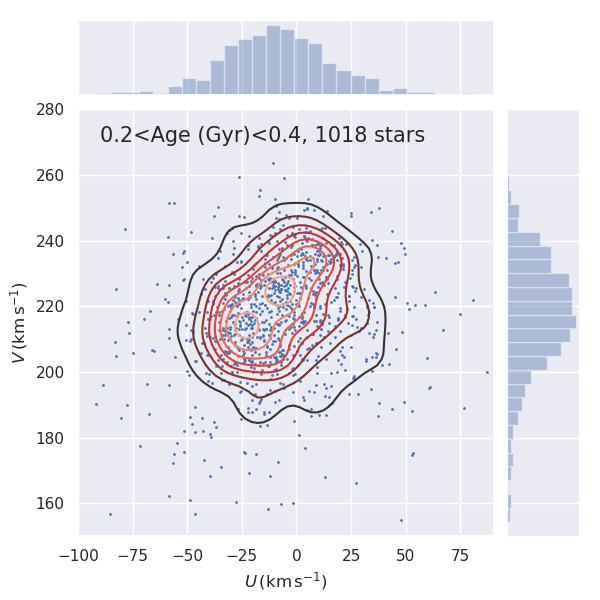
\includegraphics[width=5cm]{fig/UV/200to400Myr_z0.1kpc_hist2d.png}\\
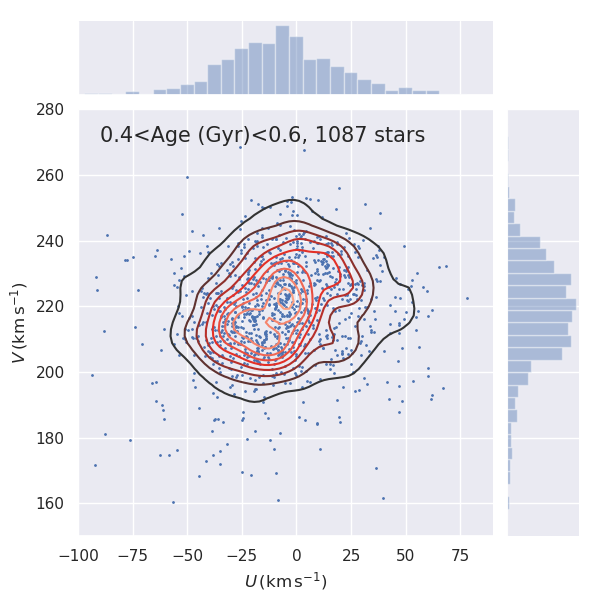
\includegraphics[width=5cm]{fig/UV/400to600Myr_z0.1kpc_hist2d.png}&
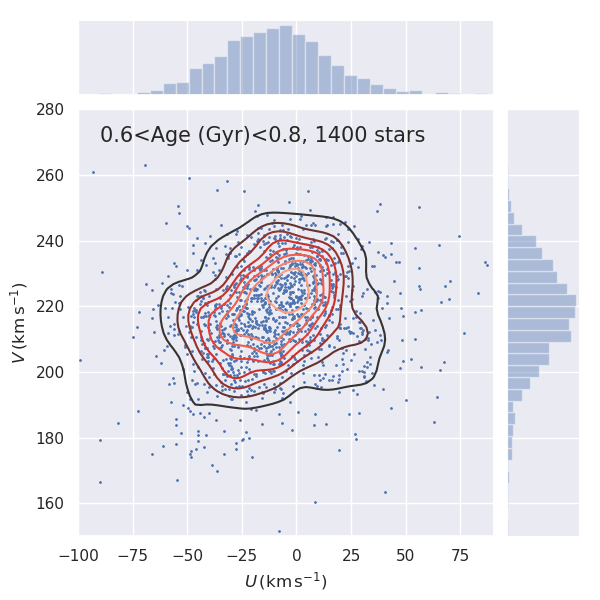
\includegraphics[width=5cm]{fig/UV/600to800Myr_z0.1kpc_hist2d.png}\\
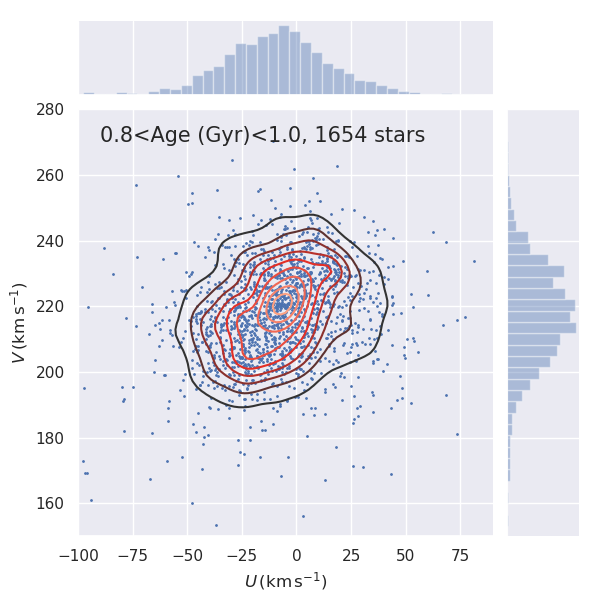
\includegraphics[width=5cm]{fig/UV/800to1000Myr_z0.1kpc_hist2d.png}&
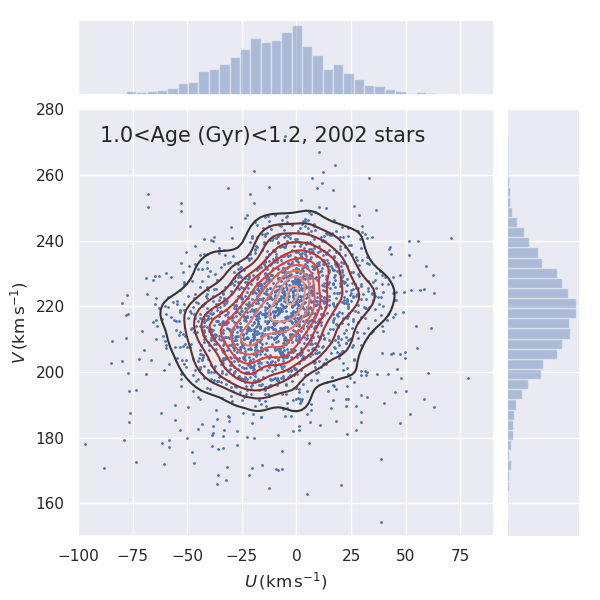
\includegraphics[width=5cm]{fig/UV/1to1.2Gyr_z0.1kpc_hist2d.png}\\
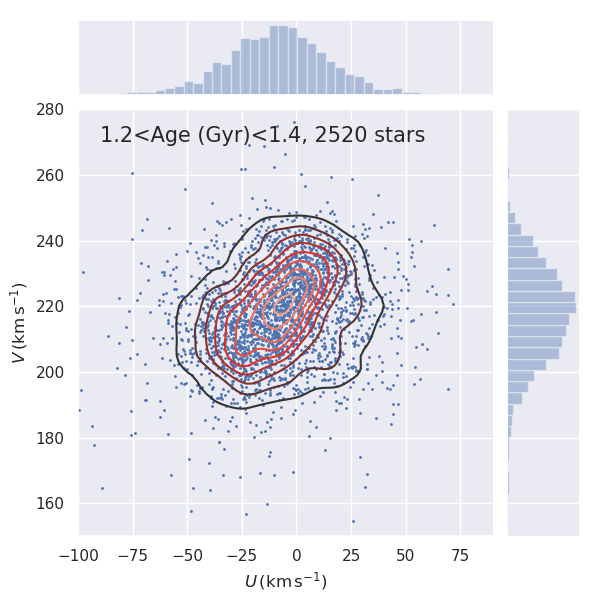
\includegraphics[width=5cm]{fig/UV/1.2to1.4Gyr_z0.1kpc_hist2d.png}&
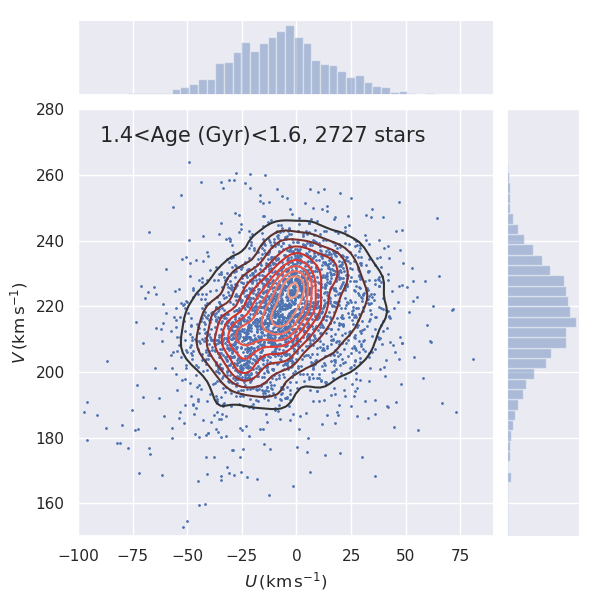
\includegraphics[width=5cm]{fig/UV/1.4to1.6Gyr_z0.1kpc_hist2d.png}\\
\end{tabular}
    \caption{太陽から1 kpc以内、年周視差の精度20\%以上、速度の観測誤差$3\,\mathrm{km\,s^{-1}}$以下の星の年齢200 Myrごとの動径方向速度$U$、方位角方向速度$V$の分布。}
    \label{hist_UV_200Myr}
\end{figure*}

\begin{figure*}[htbp]
   \centering
\begin{tabular}{cc}
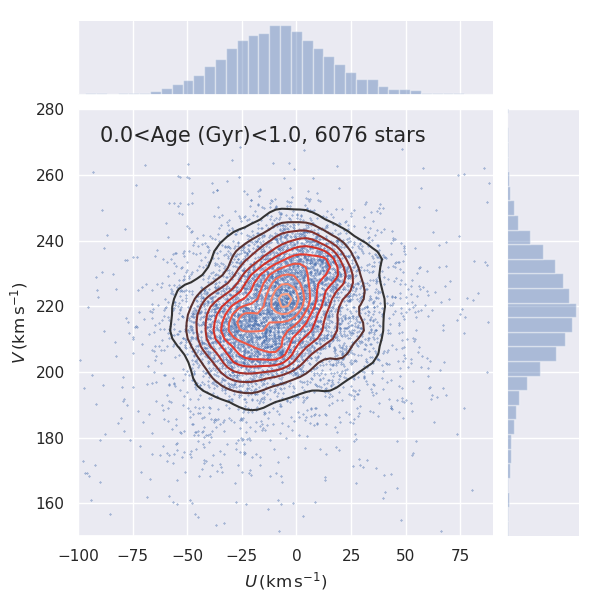
\includegraphics[width=5cm]{fig/UV/0to1Gyr_z0.1kpc_hist2d.png}&
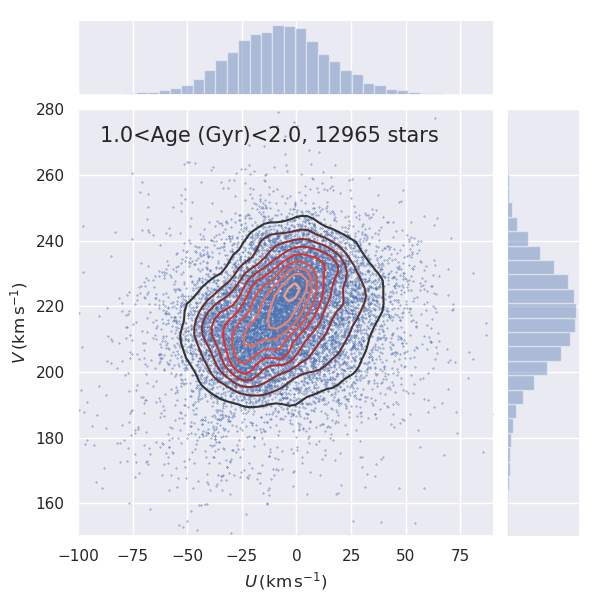
\includegraphics[width=5cm]{fig/UV/1to2Gyr_z0.1kpc_hist2d.png}\\
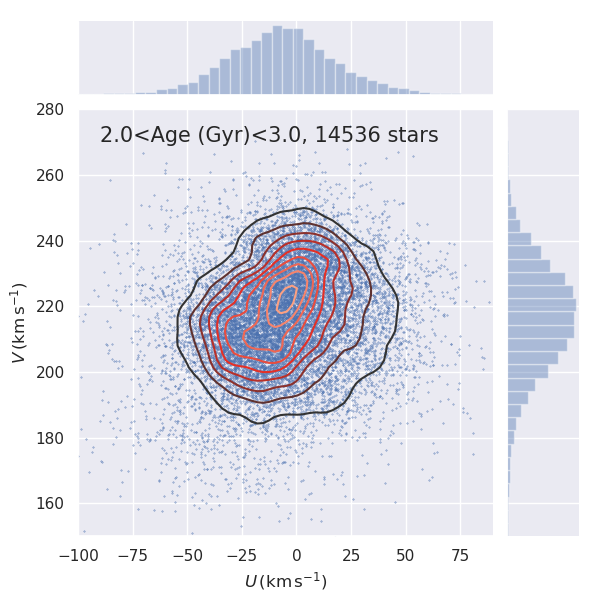
\includegraphics[width=5cm]{fig/UV/2to3Gyr_z0.1kpc_hist2d.png}&
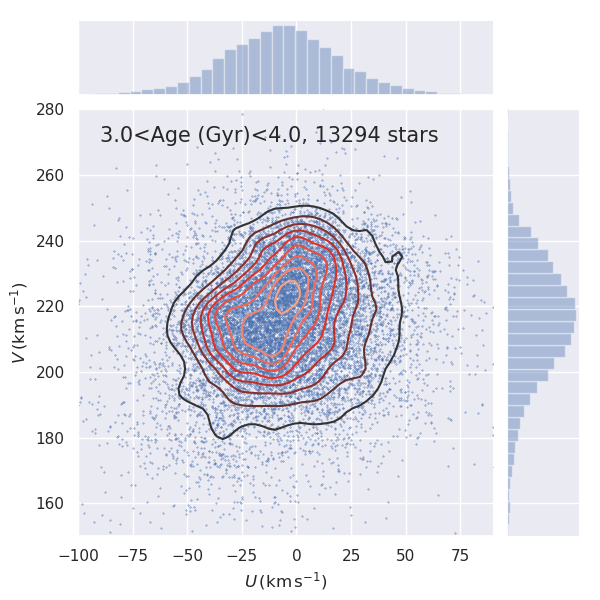
\includegraphics[width=5cm]{fig/UV/3to4Gyr_z0.1kpc_hist2d.png}\\
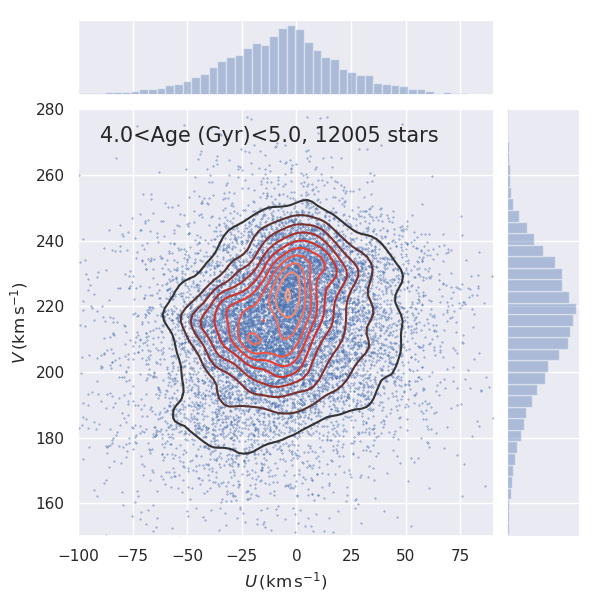
\includegraphics[width=5cm]{fig/UV/4to5Gyr_z0.1kpc_hist2d.png}&
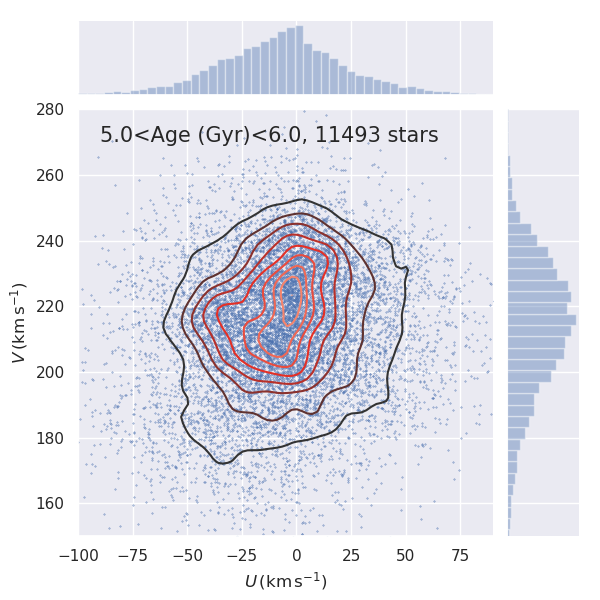
\includegraphics[width=5cm]{fig/UV/5to6Gyr_z0.1kpc_hist2d.png}\\
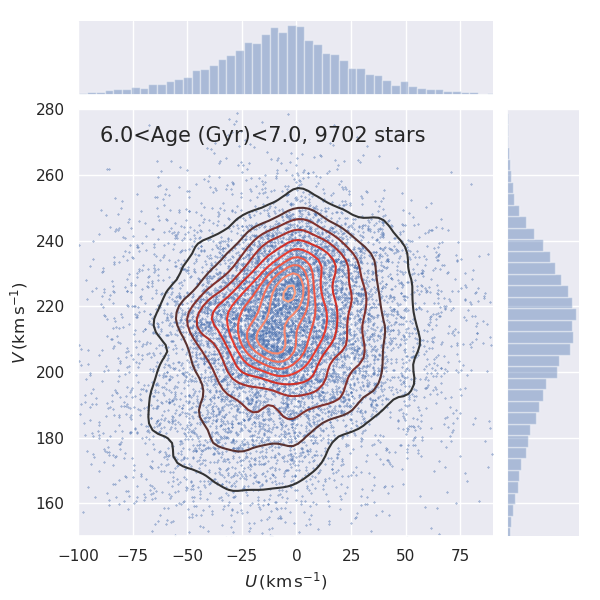
\includegraphics[width=5cm]{fig/UV/6to7Gyr_z0.1kpc_hist2d.png}&
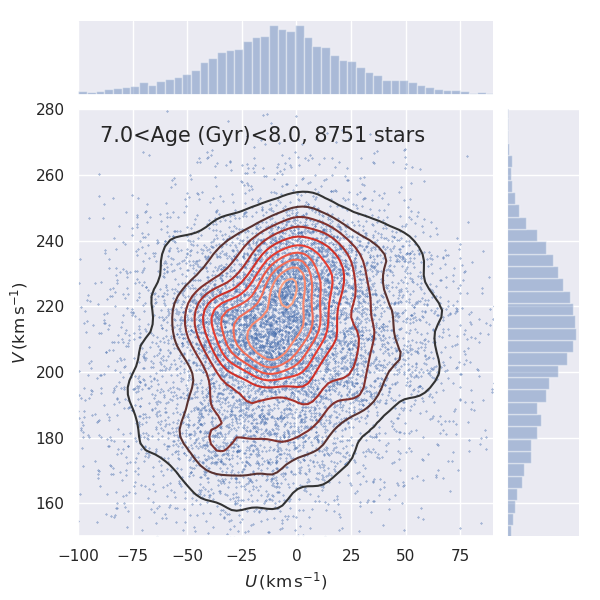
\includegraphics[width=5cm]{fig/UV/7to8Gyr_z0.1kpc_hist2d.png}\\
\end{tabular}
    \caption{太陽から1 kpc以内、年周視差の精度20\%以上、速度の観測誤差$3\,\mathrm{km\,s^{-1}}$以下の星の年齢1 Gyrごとの動径方向速度$U$、方位角方向速度$V$の分布。}
    \label{hist_UV_1Gyr}
\end{figure*}


\subsection{使用するサンプル \label{使用するサンプル}}
年周視差の相対誤差は$\varpi/\sigma_{\varpi}>5$として、20 $\%$未満としている(\cite{BJ15})。速度の観測誤差は、$\mu_l,\mu_b,v_{\mathrm{los}},\varpi$の誤差伝播を考慮して3次元速度ベクトル$v_{\mathrm{Total}}$とし、またその誤差も同様に計算して$\sigma_{v_{\mathrm{Total}}}<3\,\mathrm{km\,s^{-1}}$と制限している。本研究で用いているOort-Lindbladモデルは冷たい系を考えているため、薄い円盤星(thin disk star)に適用したい。そのため、金属量[Fe/H]$>-0.2\,\mathrm{dex})$、円盤面からの距離$|z|<100\,\mathrm{pc}$、星の年齢$\tau < 8\,\mathrm{Gyr}$のデータを用いている。星の年齢でサンプルを制限する理由は、サンプル数が少ないことと、分散が非常に大きいためである。図\ref{fig:v_sigma}はサンプルの速度と速度分散のプロットである。0 - 1 Gyrでは2 Gyrより古い星と比べて速度$\overline{V}$と速度分散の各成分で異なる傾向が見られる。表\ref{dataset}は、以上の制限をしたときのサンプル数である。

また、この観測データ解析では太陽から銀河中心までの距離は$R_0 = 8.2\pm 0.1\ \mathrm{kpc}$(\cite{BH2016})としている。また、VLBIの観測(\cite{RB04},\cite{Reid08})からいて座A$^*$に対する太陽の接線速度は$\Omega_{g,\odot} = 30.24 \pm 0.12\,\mathrm{km\,s^{-1}\ kpc^{-1}}$としている。



\begin{table}[htb]
\small
\begin{center}
\scalebox{0.87}[0.9]{
\begin{tabular}{|l|cccccccc|} \hline
    星の年齢 (Gyr) & 0 - 1 & 1 - 2 & 2 - 3 & 3 - 4 & 4 - 5 & 5 - 6 & 6 - 7 & 7 - 8\\ \hline
    $D<600\ \mathrm{pc}$のサンプル数& 4096 & 7506 & 10241 & 10416 & 9861 & 9813 & 8426 & 7716\\
    $D<700\ \mathrm{pc}$のサンプル数 & 4601 & 9044 & 11587 & 11354 & 10631 & 10480 & 8939 & 8152\\
    $D<800\ \mathrm{pc}$のサンプル数 & 5127 & 10471 & 12746 & 12134 & 11235 & 10936 & 9287 & 8436\\
    $D<900\ \mathrm{pc}$のサンプル数 & 5615 & 11821 & 13716 & 12782 & 11702 & 11283 & 9557 & 8658\\
    $D<1\ \mathrm{kpc}$のサンプル数  & 6076 & 12965 & 14537 & 13296 & 12036 & 11554 & 9768 & 8821\\ \hline
\end{tabular}
}
\caption{使用したサンプルの星の年齢と太陽からの距離の範囲でのそれぞれのサンプル数}
\end{center} \label{dataset}
\end{table}


\begin{figure*}[htbp]
	\centering
	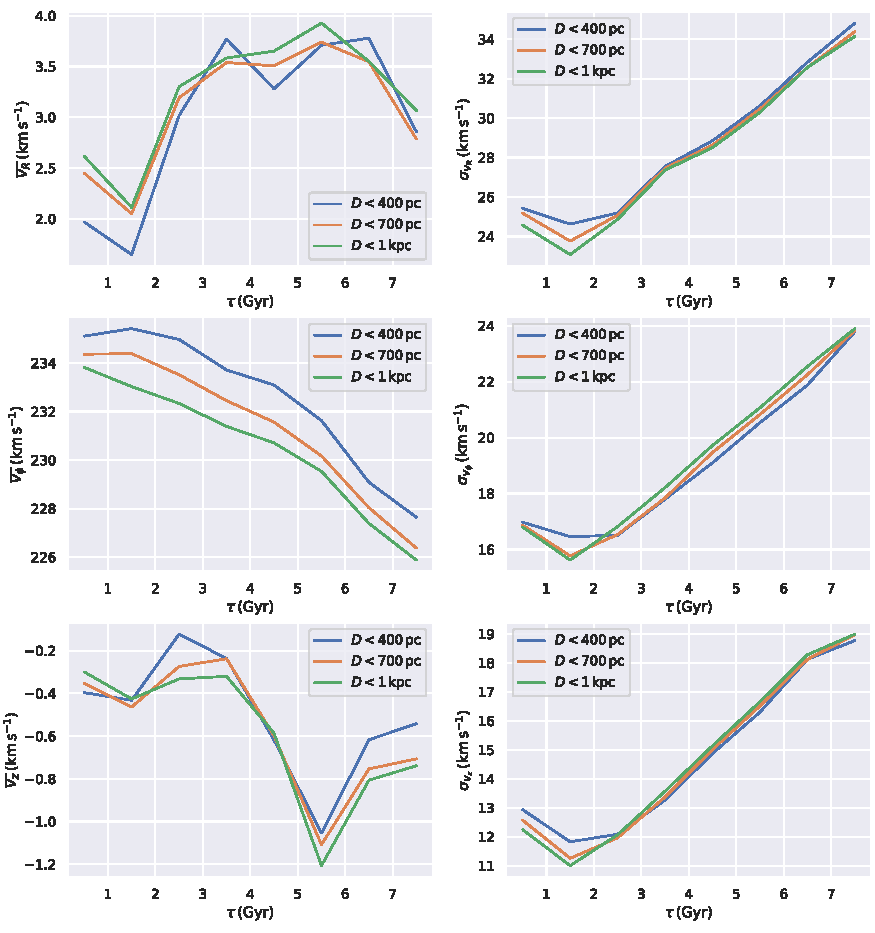
\includegraphics[width=15cm]{fig/v_sigma.pdf}
	\caption{\cite{SD18}のカタログの円筒座標系での速度と速度分散。サンプルの星の年齢を0 - 1 Gyr, 1 - 2 Gyrのように8 Gyrまでで区切っている。左側の列は各年齢での平均速度、右側の列は各年齢での速度分散の値。それぞれの線は使用したサンプルの太陽からの距離の範囲の違いである。600 pcから1 kpcまで100 pc刻みで範囲を制限している。それぞれのサンプルでほとんど違いはない。}
	\label{fig:v_sigma}
\end{figure*}


\section{観測データの解析結果 \label{観測データの解析結果}}
観測データの解析結果を示す。本研究では、大きく分けてasymmetirc drifを考慮しない従来の観測方程式(\ref{ObsEq})での解析と考慮した観測方程式(\ref{ObsEqAD})の2種類で観測データ解析を行った。

\subsection{asymmetric driftを考慮しない解析}
フィッティングパラメータは$A、\,B、\,C、\,K、\,U_{\odot}、\,V_{\odot}、\,W_{\odot}、\,\sigma_{\mu_l}、\,\sigma_{\mu_b}、\,\sigma_{v_{\mathrm{los}}}$の10個である。このときの尤度関数を求める。$\sigma_{\mu_l}、\,\sigma_{\mu_b}、\,\sigma_{v_{\mathrm{los}}}$はそれぞれ$\mu_l、\,\mu_b、\,v_{\mathrm{los}}$の平均場からの速度分散を表す。このとき尤度関数$\mathcal{L}$は
\begin{align}
\begin{aligned}
	\ln \mathcal{L} =& -\frac{1}{2}\sum_i \left(\frac{\left[\mu_{l,i} - \mu_l^{\mathrm{OL}}(l_i,b_i,\varpi_i)\right]^2}{\sigma_{\mu_l}^2 + (s_{\mu_{l,i}})^2}  + {\rm ln}\left[\sigma_{\mu_l}^2 + (s_{\mu_{l,i}})^2\right] \right. \\
	&+ \left. \frac{\left[\mu_{b,i} - \mu_b^{\mathrm{OL}}(l_i,b_i,\varpi_i)\right]^2}{\sigma_{\mu_b}^2 + (s_{\mu_{b,i}})^2}  + {\rm ln}\left[\sigma_{\mu_b}^2 + (s_{\mu_{b,i}})^2\right] \right. \\
	&+ \left. \frac{\left[v_{\mathrm{los},i} - v^{\mathrm{OL}}_{\mathrm{los}}(l_i,b_i,\varpi_i)\right]^2}{\sigma_{v_{\mathrm{los}}}^2 + (s_{v_{\mathrm{los},i}})^2} + {\rm ln}\left[\sigma_{v_{\mathrm{los}}}^2 + (s_{v_{\mathrm{los},i}})^2\right] \right)
\end{aligned}
\end{align}
と書ける。ここで、添字の$i$は$i$番目の星の値であることを示し、観測量である。また、$s_{\mu_{l,i}},s_{\mu_{b,i}},s_{v_{\mathrm{los},i}}$はそれぞれ$\mu_{l,i},\mu_{b,i},v_{\mathrm{los},i}$の観測誤差である。

%%%%%%%%%%%%%%%%%%%%%%%%%%%%%%%%%%%%5

図\ref{fig:woAD}は上記のasymmetric driftを考慮しないときの解析を観測データに対して行ったときの結果を示している。オールト定数$A,B$は太陽からの距離$D$の範囲ごとで値が0.5程度変わっている。太陽運動の銀河回転方向$V_{\odot}$は明らかに年齢依存性を持っていることがわかる。その値は0 - 1 Gyrと7 - 8 Gyrで約$6\,\mathrm{km\,s^{-1}}$増えており、1 Gyr増えるごとに約$0.75\,\mathrm{km\,s^{-1}}$増えることになる。また、オールト定数$C$は3 - 4 Gyrから4 - 5 Gyrにかけて$4\ \mathrm{km\,s^{-1}kpc}$減少している。$K$は星の年齢との間に弱い正の相関が見られる。太陽運動$U_{\odot}$は年齢が増加すると値が小さくなる傾向にある。$W_{\odot}$は年齢で大きな違いは見られない。

\begin{figure*}[htbp]
	\centering
	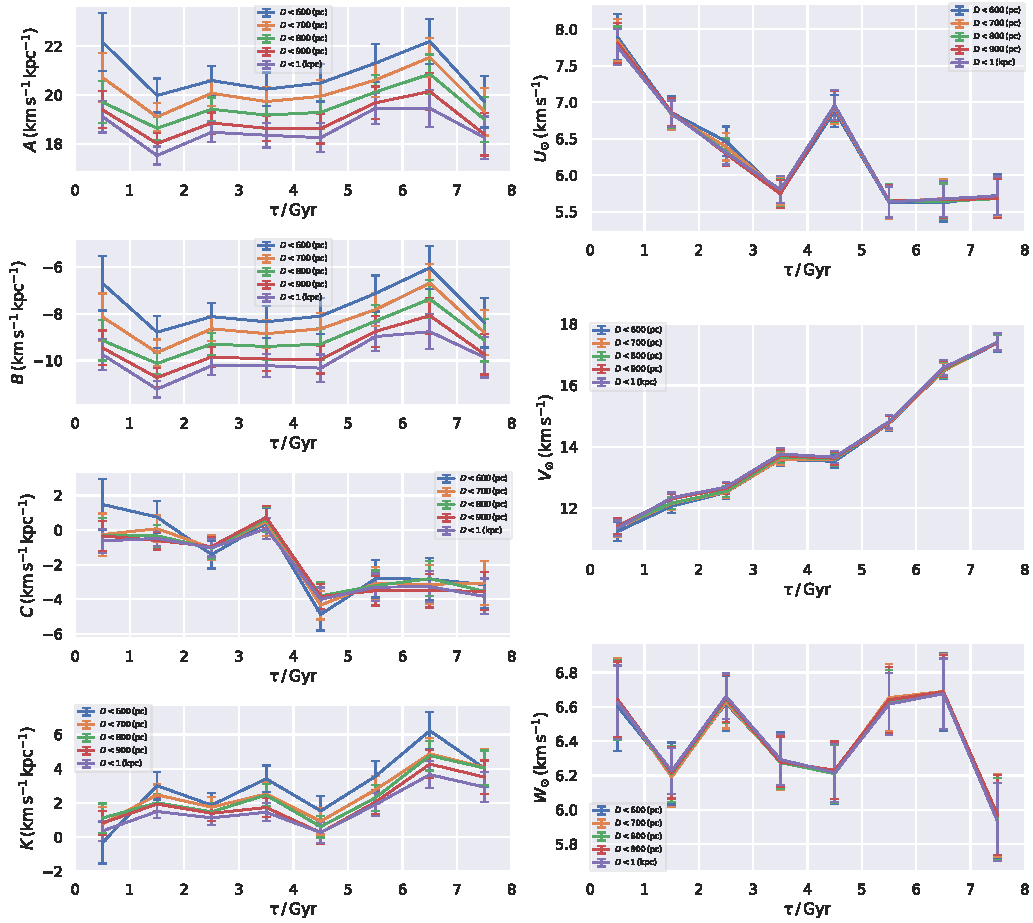
\includegraphics[width=15cm]{fig/Observation_woAD.pdf}
	\caption{asymmetric driftを考慮せずに解析したときのオールト定数と太陽運動の値。} \label{fig:woAD}
\end{figure*}




\subsection{asymmetric driftを考慮した解析}
フィッティングパラメータは同様に$A、\,B、\,C、\,K、\,U_{\odot}、\,V_{\odot}、\,W_{\odot}、\,\sigma_{\mu_l}、\,\sigma_{\mu_b}、\,\sigma_{v_{\mathrm{los}}}$の10個である。まず、以下の式で解析の準備を行う。
\begin{align}
\begin{aligned}
	D_i &= \varpi_i^{-1}\\
	R_i &= \sqrt{D_i^2 + R_0^2 - 2D_iR_0\cos{l_i}}\\
	\sin{a_i} &= \dfrac{D_i}{R_i}\sin{l_i}\\
	\cos{a_i} &= \sqrt{1 - \sin^2{a_i}}
\end{aligned}
\end{align}
asymmetric driftを考慮するために、銀河中心に対する星と太陽の速度が必要となる。$v_R$の平均値$\overline{v_R}=0$という仮定を用いると、$v_{\mathrm{c}} = R_0(A-B)$と表せる。また、接線速度は
\begin{align}
\begin{aligned}
	v_{l,i} =& \mu_{l,i}\varpi_i \kappa\\
	v_{b,i} =& \mu_{b,i}\varpi_i \kappa
\end{aligned}
\end{align}
と表せる。円筒座標系の速度は
\begin{align}
\begin{aligned}
	\left(
	\begin{array}{c}
	 	v_{R,i}\\
		v_{\phi,i}\\
		v_{\mathrm{los},i}
	\end{array}
	\right)
	=& \bf{Q}^{\mathrm{T}} \left[\bf{P}^{\mathrm{T}}
	\left(
	\begin{array}{c}
	 	v_{l,i}\\
		v_{b,i}\\
		v_{\mathrm{los},i}
	\end{array}
	\right)
	+\left(
	\begin{array}{c}
	 	U_{\odot}\\
		V_{\odot} + v_{\mathrm{c}}\\
		W_{\odot}
	\end{array}
	\right)
	\right]
\end{aligned}
\end{align}
と変換される。ここから、$v_R$の標準偏差$\sigma_R$は
\begin{align}
\begin{aligned}
	\sigma_R =& \sqrt{\frac{1}{N}\sum^N_i(v_{R,i} - \overline{v_R})^2}
\end{aligned}
\end{align}
と計算できる。asymmetric drift速度には式(\ref{AD5})を使用する。asymmetric drift速度を銀河座標系に変換すると
\begin{align}
\begin{aligned}
	\left(
	\begin{array}{c}
	 	v_{a,l}\\
		v_{a,b}\\
		v_{a,\mathrm{los}}
	\end{array}
	\right)
	=& \bf{P} \bf{Q}
	\left(
	\begin{array}{c}
	 	0\\
		v_a\\
		0
	\end{array}
	\right)
\end{aligned}
\end{align}
のようになる。表記法は\ref{sec_ObsAD}と同様である。

本解析では、$R_0$と銀河中心に対する太陽系の回転角速度$\Omega_{\odot}=V_{\phi,\odot}/R_0$について制限する。制限する値としては、$R_0=8.2\pm0.1\,\si{kpc},\Omega_{\odot}=30.24\pm0.12\,\si{km.s^{-1}.kpc}$である。このとき尤度関数$\mathcal{L}$は
\begin{align}
\begin{aligned}
	\ln \mathcal{L} =& -\frac{1}{2}\sum_i \left(\frac{\left[\mu_{l,i} - \mu_l^{\mathrm{AD}}(l_i,b_i,\varpi_i)\right]^2}{\sigma_{\mu_l}^2 + (s_{\mu_{l,i}})^2}  + {\rm ln}\left[\sigma_{\mu_l}^2 + (s_{\mu_{l,i}})^2\right] \right. \\
	&+ \frac{\left[\mu_{b,i} - \mu_b^{\mathrm{AD}}(l_i,b_i,\varpi_i)\right]^2}{\sigma_{\mu_b}^2 + (s_{\mu_{b,i}})^2}  + {\rm ln}\left[\sigma_{\mu_b}^2 + (s_{\mu_{b,i}})^2\right] \\
	&+ \frac{\left[v_{\mathrm{los},i} - v^{\mathrm{AD}}_{\mathrm{los}}(l_i,b_i,\varpi_i)\right]^2}{\sigma_{v_{\mathrm{los}}}^2 + (s_{v_{\mathrm{los},i}})^2} + {\rm ln}\left[\sigma_{v_{\mathrm{los}}}^2 + (s_{v_{\mathrm{los},i}})^2\right]\\
	&+ \frac{\left(R_0 - R_{0,\mathrm{prior}}\right)^2}{\sigma_{R_{0,\mathrm{prior}}}} + \ln{\sigma_{R_{0,\mathrm{prior}}}}\\
	&+ \left. \frac{\left(\Omega_{\odot} - \Omega_{\odot,\mathrm{prior}}\right)^2}{\sigma_{\Omega_{\odot,\mathrm{prior}}}} + \ln{\sigma_{\Omega_{\odot,\mathrm{prior}}}} \right]
\end{aligned}
\end{align}
と書ける。添字のpriorは仮定している値の平均値、$\sigma_{\mathrm{prior}}$は仮定している値の標準偏差を示す。すなわち、$R_0$の場合には$R_{0,\mathrm{prior}} = 8.2\,\si{kpc}、\,\sigma_{R_{0,\mathrm{prior}}}=0.1\,\si{kpc}$である。モデルの式については式(\ref{ObsEqAD})を参照。また、スケール長$h_R、h_{\sigma}$も制限する場合には、$R_0、\,\Omega_{\odot}$と同様に
\begin{align}
\begin{aligned}
	\ln \mathcal{L} =& -\frac{1}{2}\sum_i \left(\frac{\left[\mu_{l,i} - \mu_l^{\mathrm{AD}}(l_i,b_i,\varpi_i)\right]^2}{\sigma_{\mu_l}^2 + (s_{\mu_{l,i}})^2}  + {\rm ln}\left[\sigma_{\mu_l}^2 + (s_{\mu_{l,i}})^2\right] \right. \\
	&+ \frac{\left[\mu_{b,i} - \mu_b^{\mathrm{AD}}(l_i,b_i,\varpi_i)\right]^2}{\sigma_{\mu_b}^2 + (s_{\mu_{b,i}})^2}  + {\rm ln}\left[\sigma_{\mu_b}^2 + (s_{\mu_{b,i}})^2\right] \\
	&+ \frac{\left[v_{\mathrm{los},i} - v^{\mathrm{AD}}_{\mathrm{los}}(l_i,b_i,\varpi_i)\right]^2}{\sigma_{v_{\mathrm{los}}}^2 + (s_{v_{\mathrm{los},i}})^2} + {\rm ln}\left[\sigma_{v_{\mathrm{los}}}^2 + (s_{v_{\mathrm{los},i}})^2\right]\\
	&+ \frac{\left(R_0 - R_{0,\mathrm{prior}}\right)^2}{\sigma_{R_{0,\mathrm{prior}}}} + \ln{\sigma_{R_{0,\mathrm{prior}}}}\\
	&+ \frac{\left(\Omega_{\odot} - \Omega_{\odot,\mathrm{prior}}\right)^2}{\sigma_{\Omega_{\odot,\mathrm{prior}}}} + \ln{\sigma_{\Omega_{\odot,\mathrm{prior}}}}\\
	&+ \frac{\left(h_R - h_{R,\mathrm{prior}}\right)^2}{\sigma_{h_{R,\mathrm{prior}}}} + \ln{\sigma_{h_{R,\mathrm{prior}}}}\\
	&+ \left. \frac{\left(h_{\sigma} - h_{\sigma,\mathrm{prior}}\right)^2}{\sigma_{h_{\sigma,\mathrm{prior}}}} + \ln{\sigma_{h_{\sigma,\mathrm{prior}}}} \right)
\end{aligned}
\end{align}
となる。

%%%%%%%%%%%%%%%%%%%%%%%%%%%%%%%%

asymmetric driftを考慮したときの観測方程式(\ref{ObsEq})を用いた解析の結果を示す。asymmetric driftの式には式\ref{AD2}を使用している。asymmetric driftを考慮した解析では動径方向の密度と速度分散のスケール長$h_R,h_{\sigma}$の制限の仕方で大きく3種類の解析を行っている(表\ref{scalelength})。$h_{\sigma}=2h_R$としている。解析の結果、これら全ての解析に共通して$A,B,U_{\odot},V_{\odot},W_{\odot}$は星の年齢に対して依存性を持っている。特に、$V_{\odot}$ははっきりとした年齢依存性が見られる。$V_{\odot}$の年齢依存性については、asymmetric driftを考慮しない解析と同様の傾向が見られるが、asymmetric driftを考慮した場合よりも全年齢において約$1\,\mathrm{km\,s^{-1}}$小さくなっている。

\begin{table}
\begin{center}
%\scalebox{0.5}
%\scriptsize
%\footnotesize
%\small
\begin{tabular}{c|l|c|c|c} \hline
 \rowcolor{LightCyan}
 解析名 & Reference & $h_R\ \mathrm{(kpc)}$ & $h_{\sigma}\ \mathrm{(kpc)}$ & 図\\
 \hline
  1-a & \multirow{3}{*}{\cite{Piffl14}} & 2.68 & 9 & \ref{figObs1a}\\
  1-b && 2.68 & $(2\pm 0.5)h_R$ & \\
  1-c && 2.68 & $(2\pm 0.5)h_R$ & \tabularnewline[\doublerulesep]
 \hline
  2-a & \multirow{3}{*}{\cite{SB15}} & 3.45 & 7.8 & \ref{figObs2a}\\
  2-b && 3.45 & $(2\pm 0.5)h_R$ & \ref{figObs2b}\\
  2-c && 3.45 & $(2\pm 0.5)h_R$ & \ref{figObs2c} \tabularnewline[\doublerulesep]
 \hline
  3-a & \multirow{3}{*}{\cite{BP15}} & 3.66 & $2h_R$ & \ref{figObs3a}\\
  3-b && 3.66 & $(2\pm 0.5)h_R$ & \ref{figObs3b}\\
  3-c && 3.66 & $(2\pm 0.5)h_R$ & \ref{figObs3c} \tabularnewline[\doublerulesep]
 \hline
  4 & \cite{BP15} & $(3.66 \pm 1.0) + 8 - \tau\ (\mathrm{Gyr})$ & $(2\pm 0.5)h_R$ & \ref{figObs4}\\
 \hline
  5 & \cite{BH2016} & $(2.6 \pm 1.0) + 8 - \tau\ (\mathrm{Gyr})$ & $(2\pm 0.5)h_R$ & \ref{figObs5}\\
 \hline
\end{tabular} \label{scalelength}
\caption{観測データのasymmetric driftを考慮した解析を行った際に仮定したスケール長。}
\end{center}
\end{table}


%%%%%%%%%%%%%%%%%%%%%%%%%%%%%%%%%%%%%%%%%%%%%%%%%%%%%%%%%%%%%%%%%%%%%%%%%%%%%%%%%%%%%%%%%%%%%%%%%%%%%%%%
%%%%%%%%%%%%%%%%%%%%%%%%%%%%%%%%%%%%%%%%%%%%%%%%%%%%%%%%%%%%%%%%%%%%%%%%%%%%%%%%%%%%%%%%%%%%%%%%%%%%%%%%

\begin{figure*}[htbp]
   \centering
\begin{tabular}{cc}
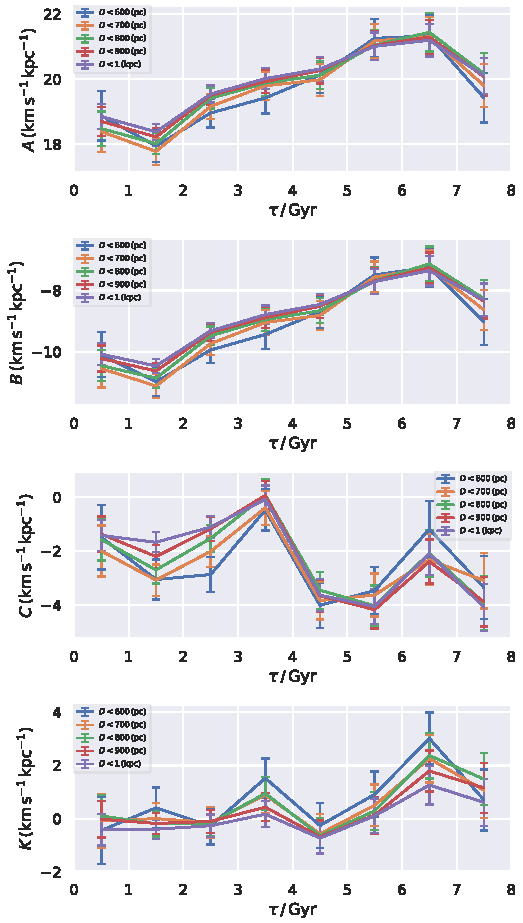
\includegraphics[width=7cm]{fig/ABCK_1a.pdf}
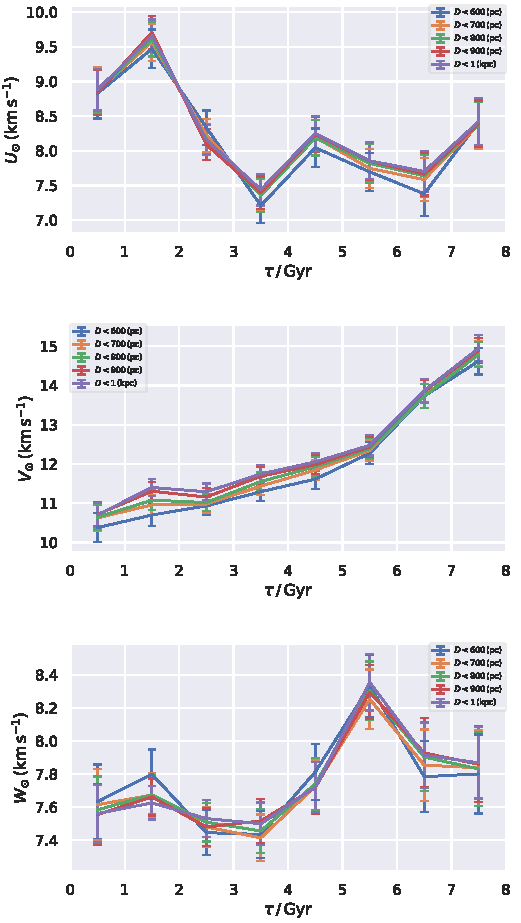
\includegraphics[width=7cm]{fig/UVW_1a.pdf}
\end{tabular}
    \caption{(解析1-a) $h_R=2.68\,\mathrm{kpc}, h_{\sigma}=9\,\mathrm{kpc}$として解析したときのオールト定数と太陽運動の値。}
    \label{figObs1a}
\end{figure*}

図\ref{tri1a_0-1}を見ると、$A,B$間で非常に強い相関が見られる。また、若い星の方が古い星よりも$A,B$と$V_{\odot}$との間に負の相関、$C,K$と$U_{\odot}$との間にも弱い負の相関が見られる。

\begin{figure*}[htbp]
\begin{center}
	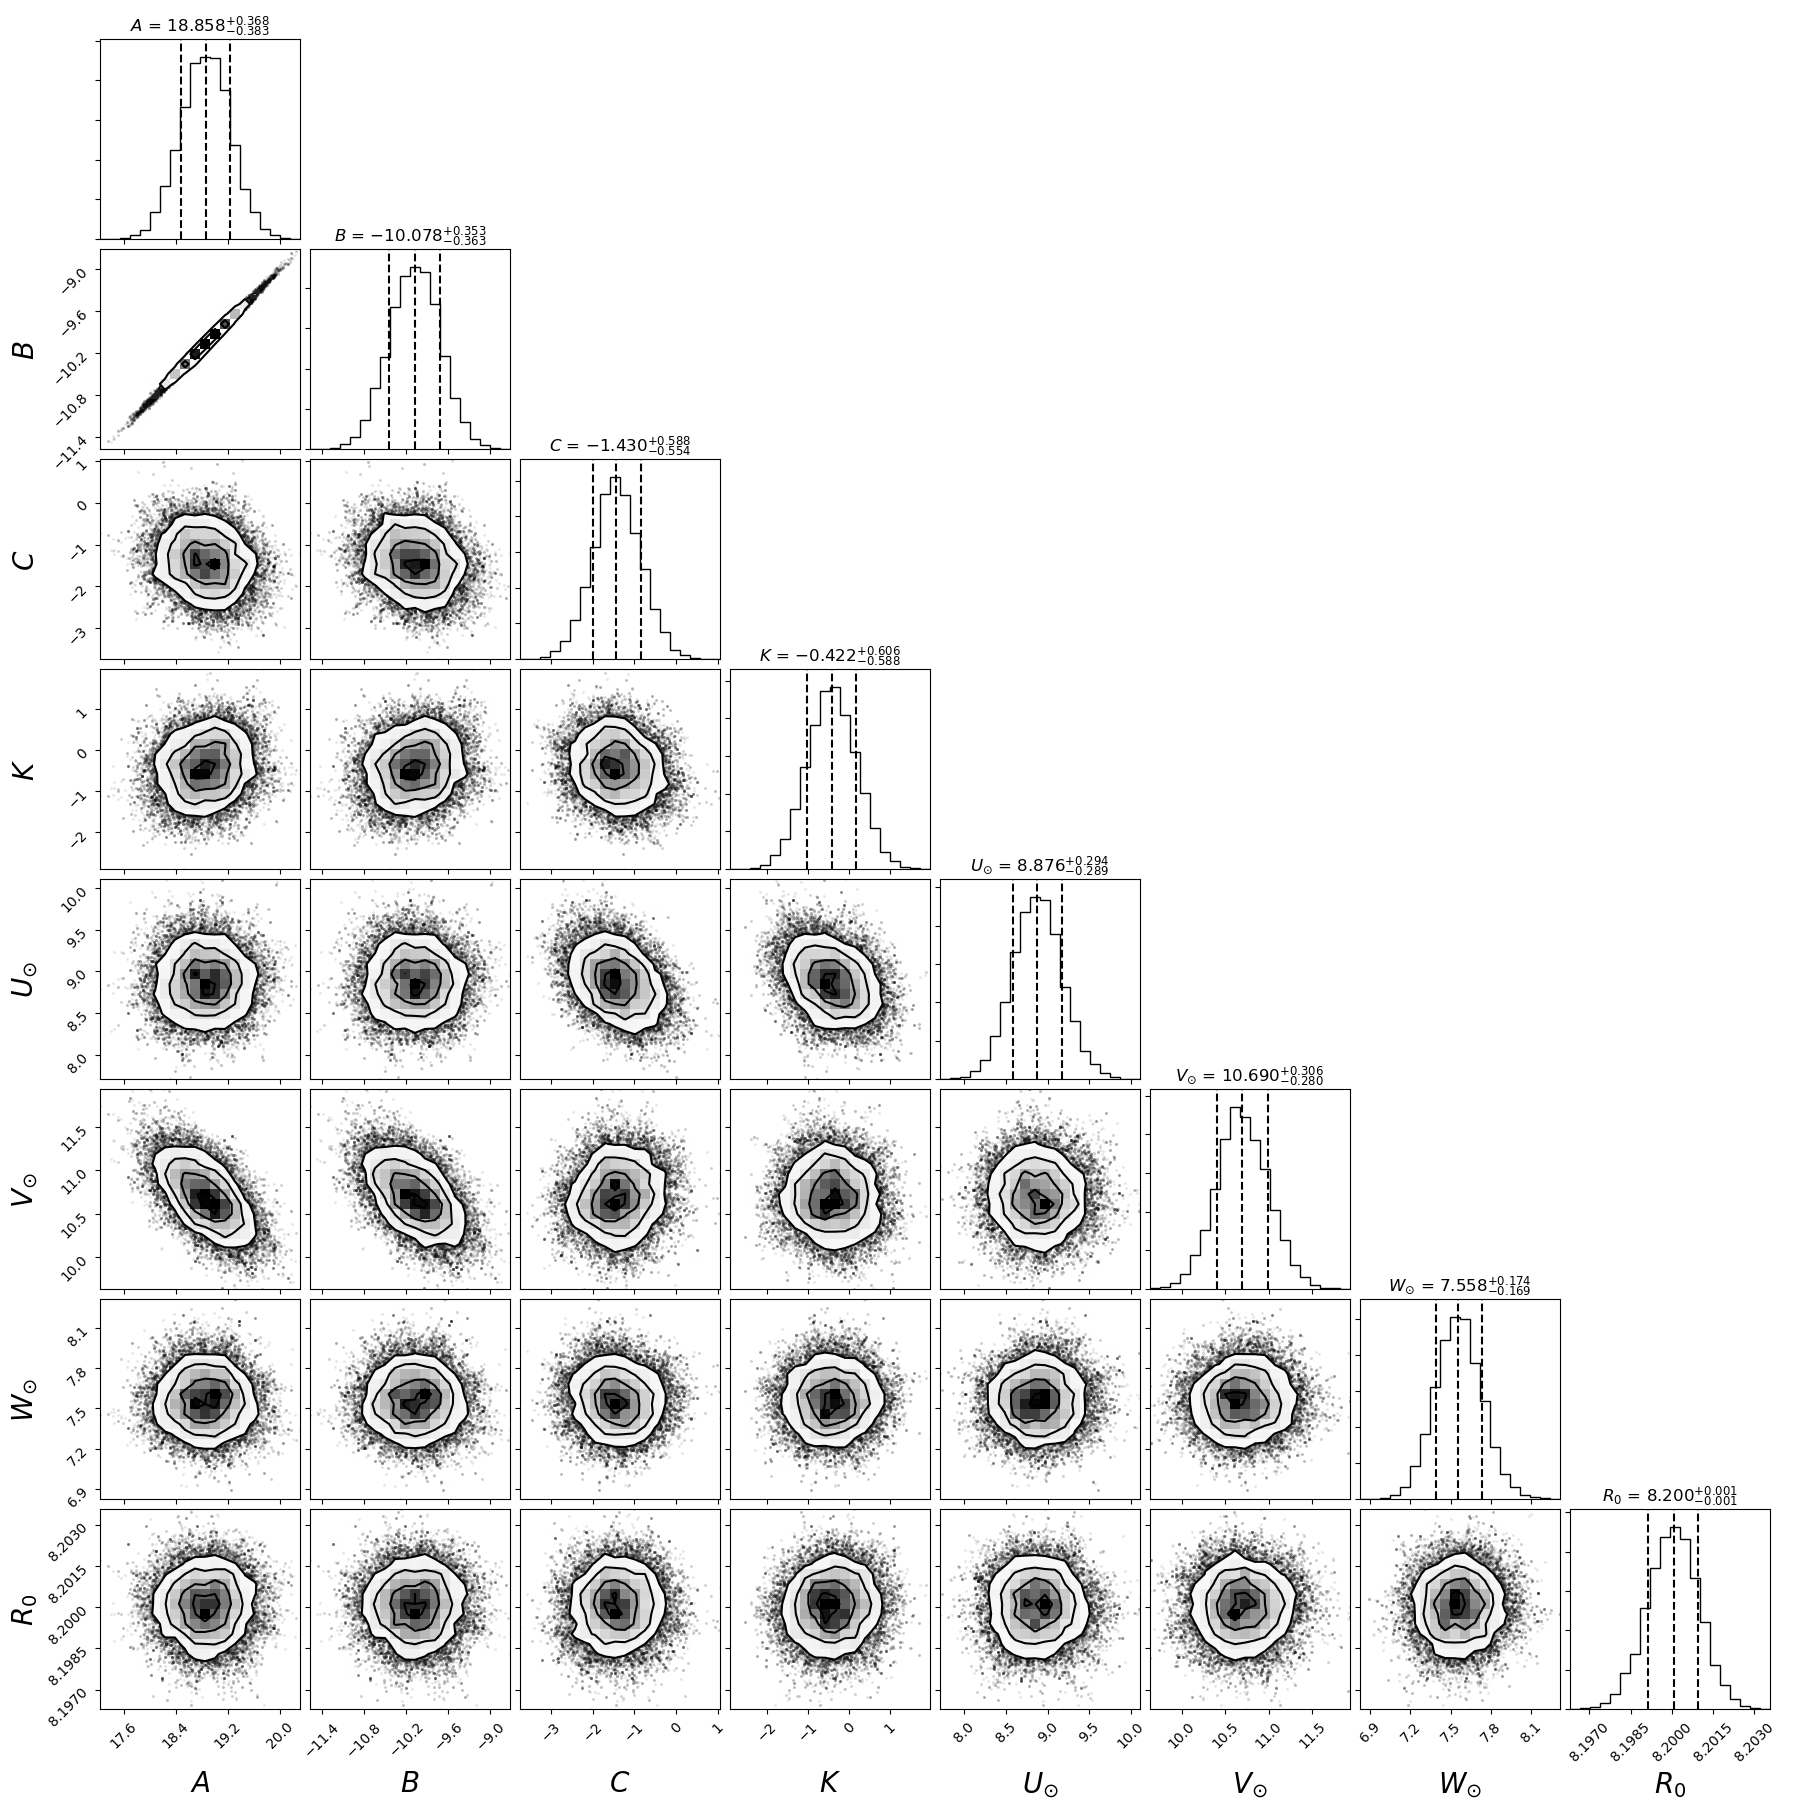
\includegraphics[width=14cm]{fig/1a/trinagle_walker60_Nrun3000_Nburn2000_withscatter_0to1Gyr_1kpc_6076stars_newModel_23.png}
	\caption{(解析1-a) 0 - 1 Gyrのサンプルの解析結果のコーナープロット。各パラメータの事後確率分布とそれぞれのパラメータ間の相関を表している。}
	\label{tri1a_0-1}
\end{center}
\end{figure*}

%%%%%%%%%%%%%%%%%%%%%%%%%%%%%%%%%%%%%%%%%%%%%%%%%%%%%%%%%%%%%%%%%%%%%%%%%%%%%%%%%%%%%%%%%%%%%%%%%%%%%%%%
%%%%%%%%%%%%%%%%%%%%%%%%%%%%%%%%%%%%%%%%%%%%%%%%%%%%%%%%%%%%%%%%%%%%%%%%%%%%%%%%%%%%%%%%%%%%%%%%%%%%%%%%

\begin{figure*}[htbp]
   \centering
\begin{tabular}{cc}
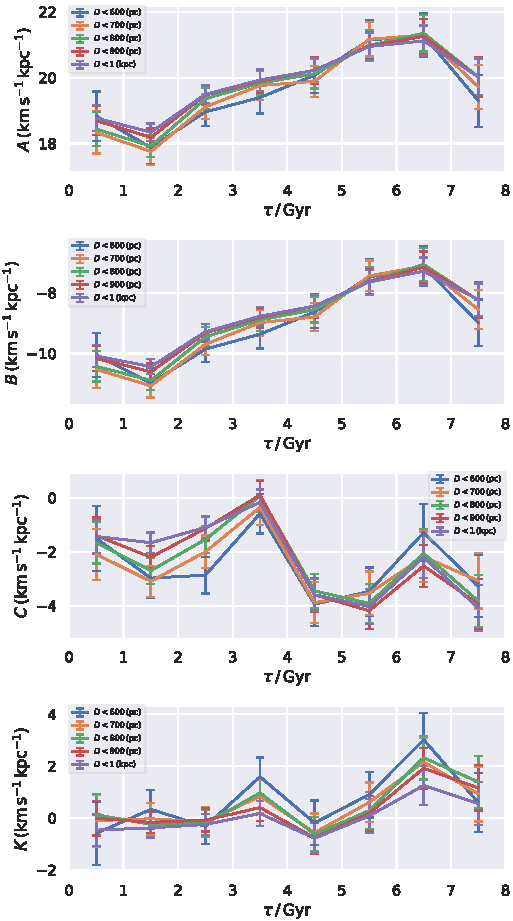
\includegraphics[width=7cm]{fig/ABCK_2a.pdf}
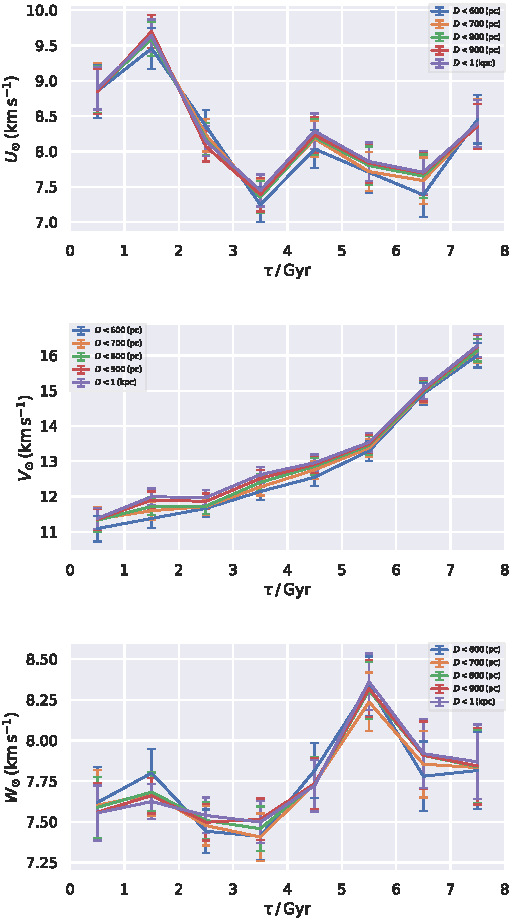
\includegraphics[width=7cm]{fig/UVW_2a.pdf}
\end{tabular}
    \caption{(解析2-a) $h_R=3.66\,\mathrm{kpc}, h_{\sigma}=2h_R$として解析したときのオールト定数と太陽運動の値。サンプルの取り方は太陽からの距離の範囲を変えている。}
    \label{figObs2a}
\end{figure*}

\begin{figure*}[htbp]
   \centering
\begin{tabular}{cc}
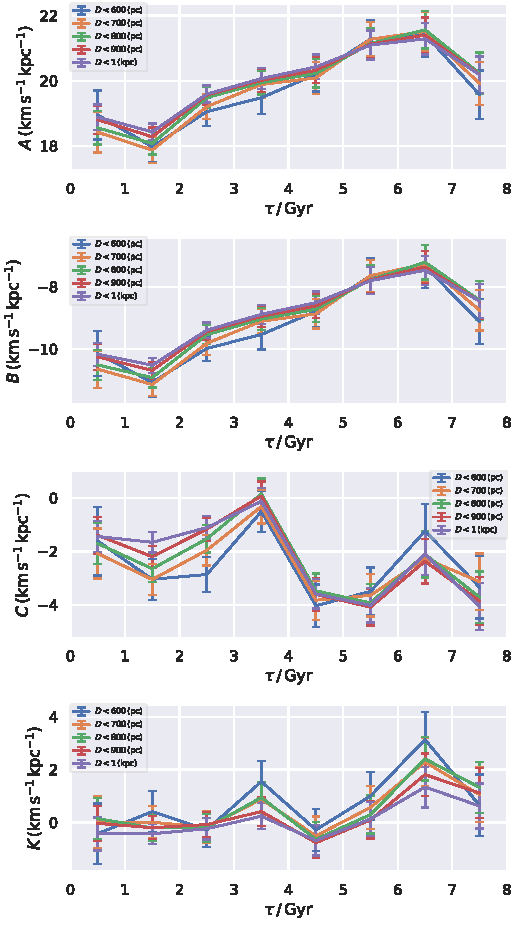
\includegraphics[width=7cm]{fig/ABCK_2b.pdf}
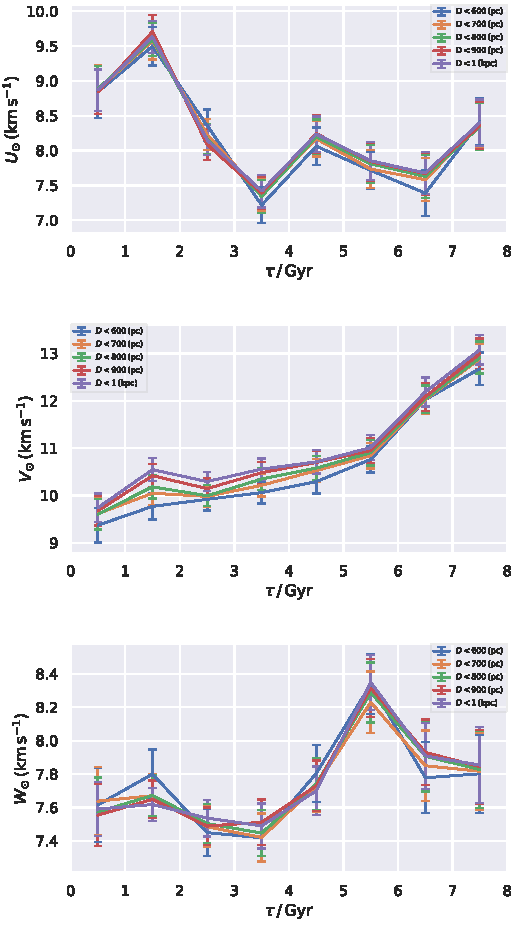
\includegraphics[width=7cm]{fig/UVW_2b.pdf}
\end{tabular}
    \caption{(解析2-b) $h_R=3.66\pm 1.0\,\mathrm{kpc},h_{\sigma}=2h_R$として解析したときのオールト定数と太陽運動の値。サンプルの取り方は太陽からの距離の範囲を変えている。}
    \label{figObs2b}
\end{figure*}

\begin{figure*}[htbp]
   \centering
\begin{tabular}{cc}
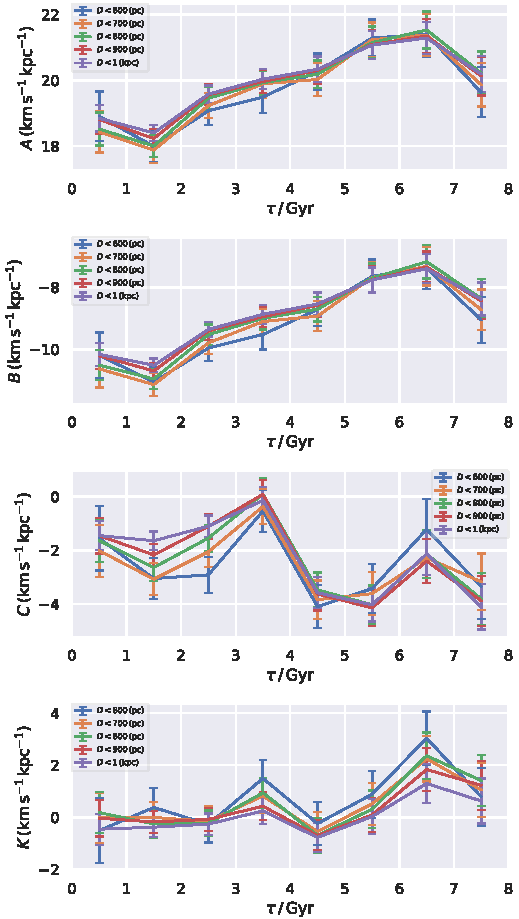
\includegraphics[width=7cm]{fig/ABCK_2c.pdf}
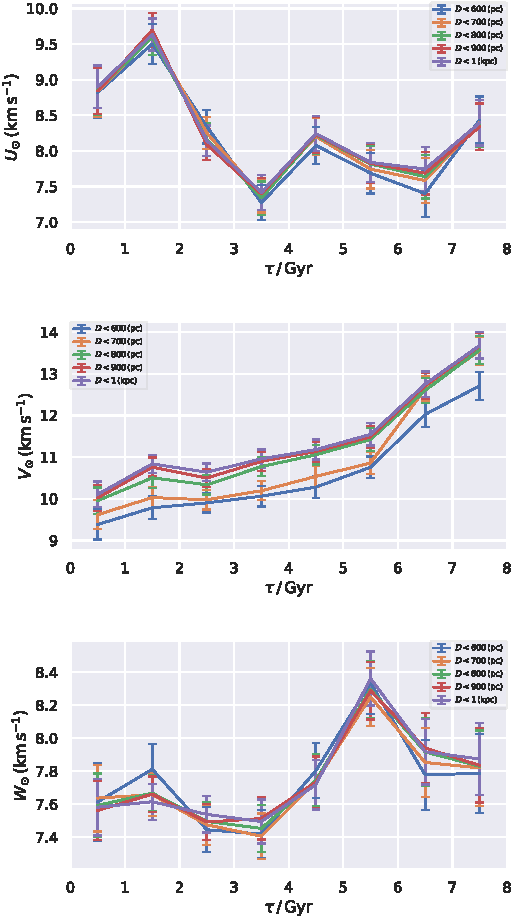
\includegraphics[width=7cm]{fig/UVW_2c.pdf}
\end{tabular}
    \caption{(解析2-c) $h_R=3.66\pm 1.0\,\mathrm{kpc},h_{\sigma}=(2\pm 0.5)h_R$として解析したときのオールト定数と太陽運動の値。サンプルの取り方は太陽からの距離の範囲を変えている。}
    \label{figObs2c}
\end{figure*}

%%%%%%%%%%%%%%%%%%%%%%%%%%%%%%%%%%%%%%%%%%%%%%%%%%%%%%%%%%%%%%%%%%%%%%%%%%%%%%%%%%%%%%%%%%%%%%%%%%%%%%%%
%%%%%%%%%%%%%%%%%%%%%%%%%%%%%%%%%%%%%%%%%%%%%%%%%%%%%%%%%%%%%%%%%%%%%%%%%%%%%%%%%%%%%%%%%%%%%%%%%%%%%%%%

\begin{figure*}[htbp]
   \centering
\begin{tabular}{cc}
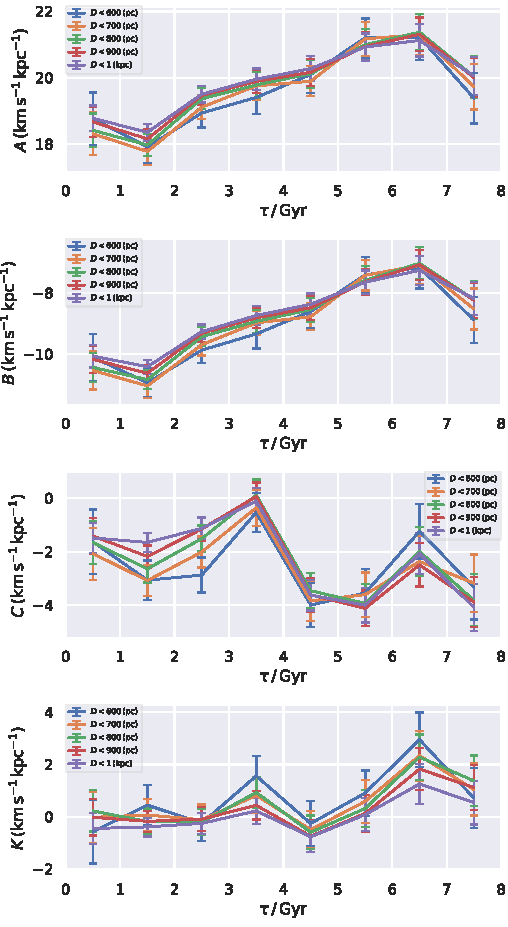
\includegraphics[width=7cm]{fig/ABCK_3a.pdf}
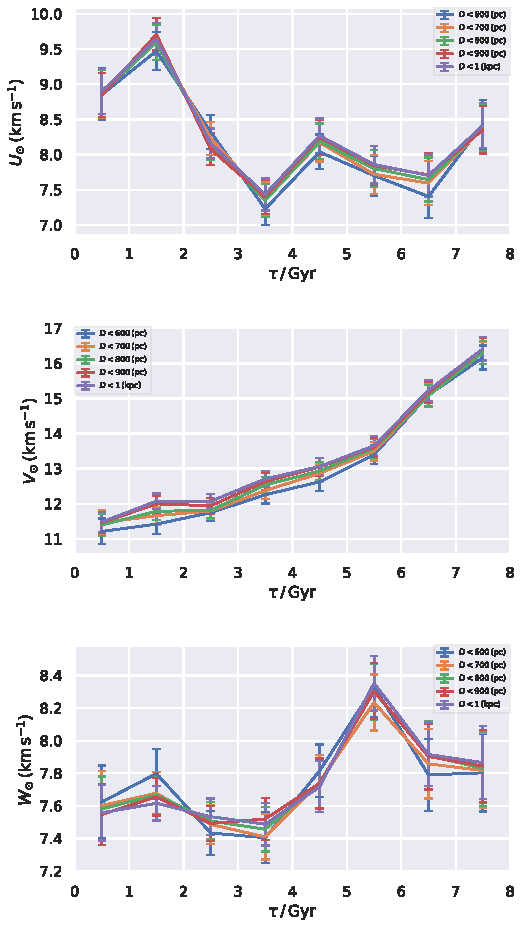
\includegraphics[width=7cm]{fig/UVW_3a.pdf}
\end{tabular}
    \caption{(解析3-a) $h_R=3.66\,\mathrm{kpc}, h_{\sigma}=2h_R$として解析したときのオールト定数と太陽運動の値。サンプルの取り方は太陽からの距離の範囲を変えている。}
    \label{figObs3a}
\end{figure*}

\begin{figure*}[htbp]
   \centering
\begin{tabular}{cc}
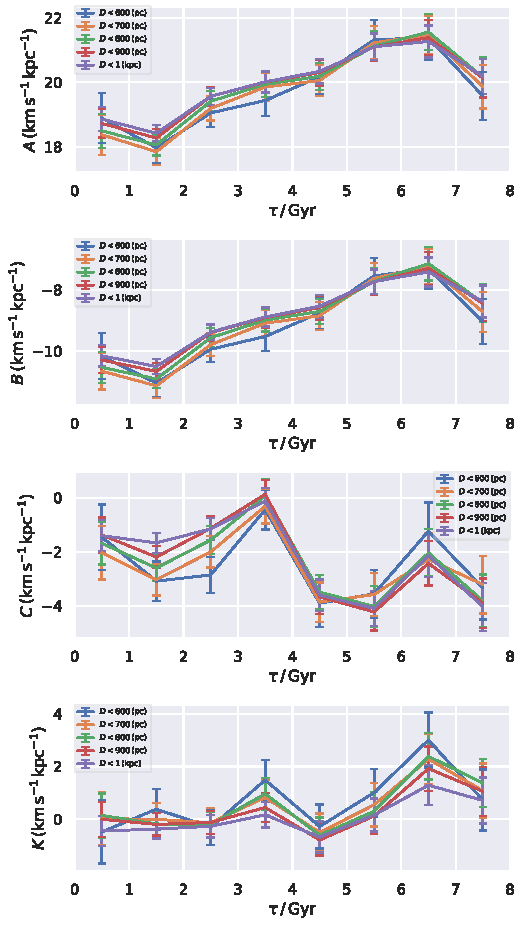
\includegraphics[width=7cm]{fig/ABCK_3b.pdf}
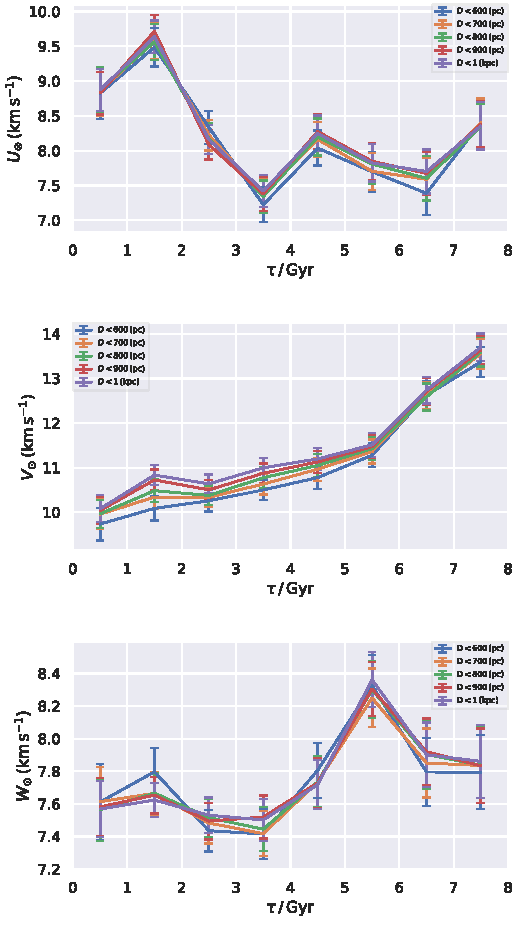
\includegraphics[width=7cm]{fig/UVW_3b.pdf}
\end{tabular}
    \caption{(解析3-b) $h_R=3.66\pm 1.0\,\mathrm{kpc},h_{\sigma}=2h_R$として解析したときのオールト定数と太陽運動の値。サンプルの取り方は太陽からの距離の範囲を変えている。}
    \label{figObs3b}
\end{figure*}

\begin{figure*}[htbp]
   \centering
\begin{tabular}{cc}
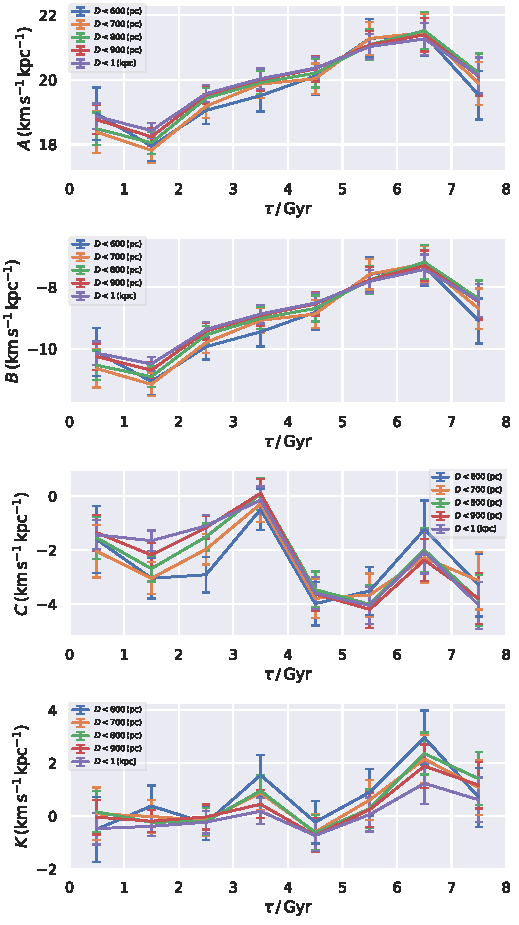
\includegraphics[width=7cm]{fig/ABCK_3c.pdf}
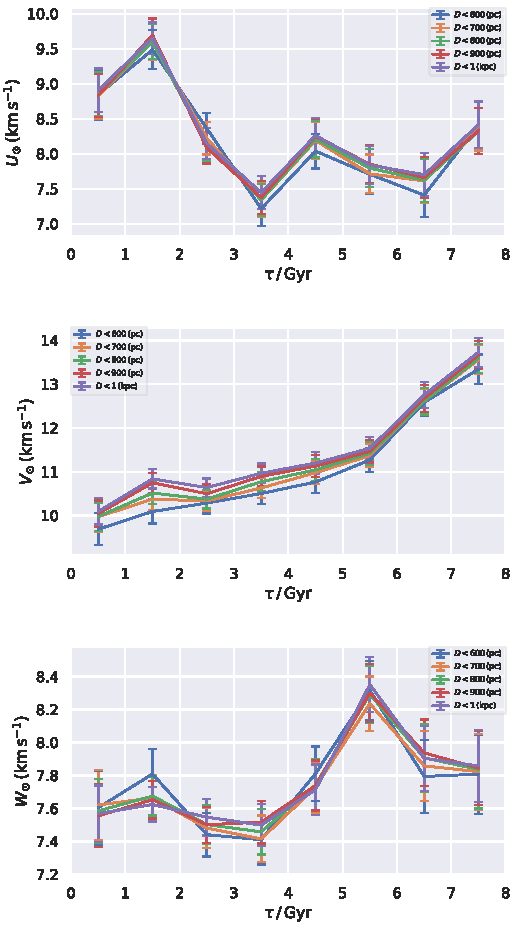
\includegraphics[width=7cm]{fig/UVW_3c.pdf}
\end{tabular}
    \caption{(解析3-c) $h_R=3.66\pm 1.0\,\mathrm{kpc},h_{\sigma}=(2\pm 0.5)h_R$として解析したときのオールト定数と太陽運動の値。サンプルの取り方は太陽からの距離の範囲を変えている。}
    \label{figObs3c}
\end{figure*}


%%%%%%%%%%%%%%%%%%%%%%%%%%%%%%%%%%%%%%%%%%%%%%%%%%%%%%%%%%%%%%%%%%%%%%%%%%%%%%%%%%%%%%%
%%%%%%%%%%%%%%%%%%%%%%%%%%%%%%%%%%%%%%%%%%%%%%%%%%%%%%%%%%%%%%%%%%%%%%%%%%%%%%%%%%%%%%%
%%%%%%%%%%%%%%%%%%%%%%%%%%%%%%%%%%%%%%%%%%%%%%%%%%%%%%%%%%%%%%%%%%%%%%%%%%%%%%%%%%%%%%%

\begin{figure*}[htbp]
   \centering
\begin{tabular}{cc}
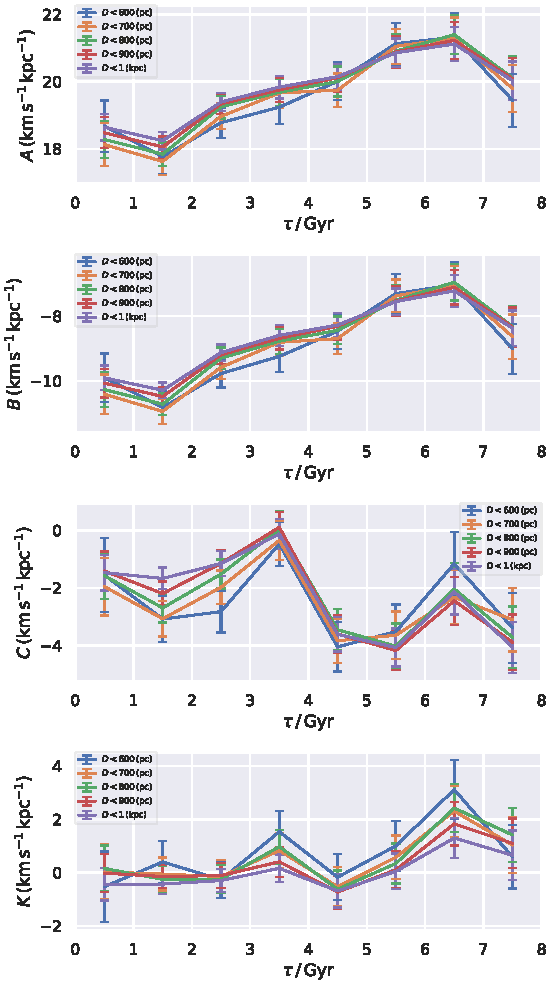
\includegraphics[width=7cm]{fig/ABCK_4.pdf}
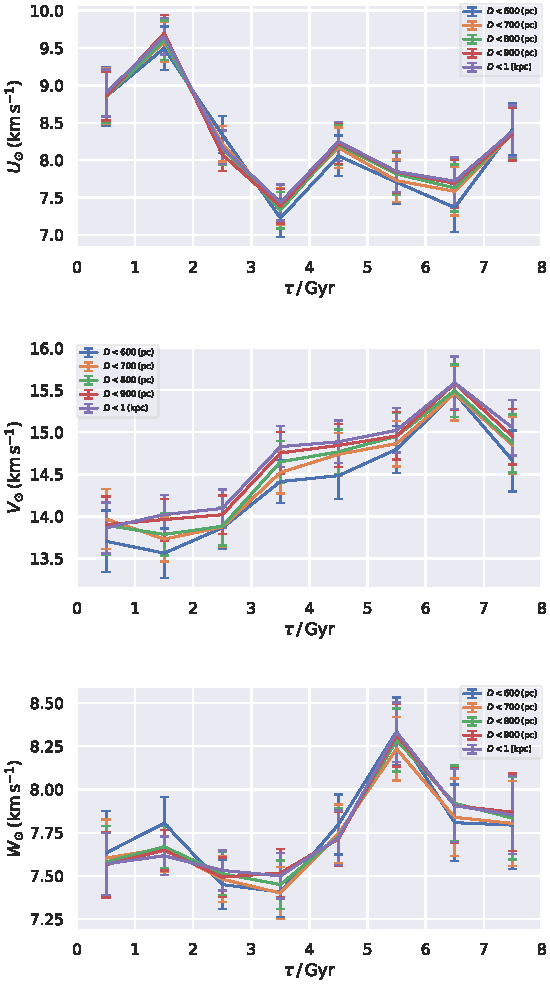
\includegraphics[width=7cm]{fig/UVW_4.pdf}
\end{tabular}
    \caption{(解析4) $(3.66 \pm 1.0) + 8 - \tau\ (\mathrm{Gyr}), h_{\sigma} = (2\pm 0.5)h_R$として解析したときのオールト定数と太陽運動の値。サンプルの取り方は太陽からの距離の範囲を変えている。}
    \label{figObs4}
\end{figure*}

\begin{figure*}[htbp]
   \centering
\begin{tabular}{cc}
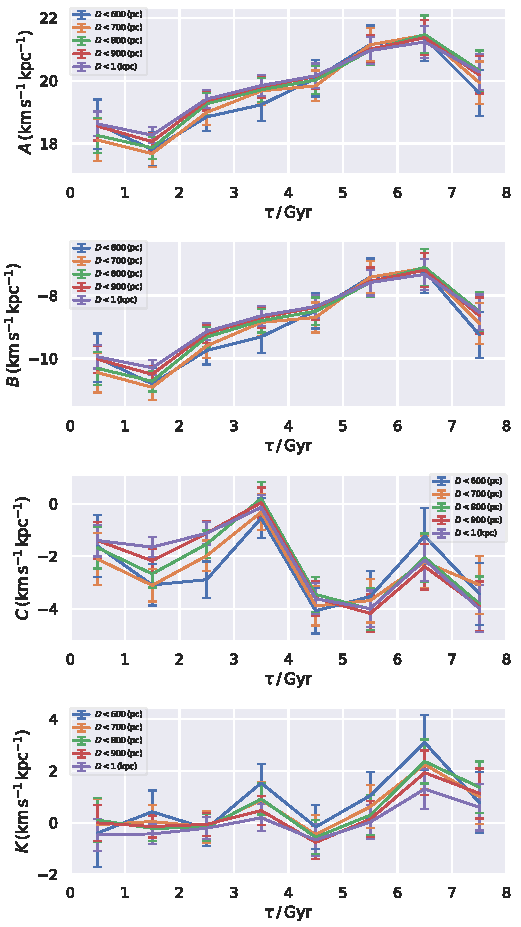
\includegraphics[width=7cm]{fig/ABCK_5.pdf}
\includegraphics[width=7cm]{fig/UVW_5.pdf}
\end{tabular}
    \caption{(解析5) $(2.6 \pm 1.0) + 8 - \tau\ (\mathrm{Gyr}), h_{\sigma} = (2\pm 0.5)h_R$解析したときのオールト定数と太陽運動の値。サンプルの取り方は太陽からの距離の範囲を変えている。}
    \label{figObs5}
\end{figure*}

%%%%%%%%%%%%%%%%%%%%%%%%%%%%%%%%%%%%%%%%%%%%%%%%%%%%%%%%%%%%%%%%%%%%%%%%%%%%%%%%%%%%%%%
%%%%%%%%%%%%%%%%%%%%%%%%%%%%%%%%%%%%%%%%%%%%%%%%%%%%%%%%%%%%%%%%%%%%%%%%%%%%%%%%%%%%%%%
%%%%%%%%%%%%%%%%%%%%%%%%%%%%%%%%%%%%%%%%%%%%%%%%%%%%%%%%%%%%%%%%%%%%%%%%%%%%%%%%%%%%%%%

\section{解析結果のまとめ}
図\ref{multi}は太陽から1 kpc以内のサンプルを使用したときのasymmtric drift無し(no AD)とasymmetric drift有りの各解析のプロットである。この結果を見ると、全ての解析パラメータにおいてasymmetric drift無しと有りとの解析で明確に違いが出た。オールト定数$A,B,C,K$と太陽運動$U_{\odot},W_{\odot}$については全てのasyymetric drift有りの解析でほぼ同じ結果となった。しかし、太陽運動の銀河回転成分$V_{\odot}$のみはasymmetric drift有りの解析の中でも結果に違いが出た。これは、スケール長(表\ref{scalelength})の違いによるものだと考えられる。
\begin{figure*}[htbp]
\begin{center}
	\includegraphics[width=15cm]{fig/multi/multi.pdf}
	\caption{太陽から1 kpc以内のサンプルを使用したときのasymmtric drift無し(no AD)とasymmetric drift有りの各解析のプロット。各線の色と解析方法の対応関係のラベルは図の上部に記載している。解析方法の詳細は表\ref{scalelength}を参照。}
	\label{multi}
\end{center}
\end{figure*}